\chapter{Implementation}\label{cap:implementation}

After the chapter where the software architecture was detailed, this chapter is focused on explaining how such architecture was implemented, as while the first describes the structure and organization, this one focuses on the technical actions adopted to make this structure work.

For a more structured and detailed analysis, this chapter has been divided into specific sections for each system component. They are:

\begin{itemize}
    \item \textbf{Database implementation}: This section will address the technical details of the database design and how information is stored and retrieved.
    
    \item \textbf{Implementation of the data receiving module}: This section will detail how data is received, validated, and processed before being stored and made available to users.
    
    \item \textbf{API Implementation}: Here, the structure of the \gls{API} will be discussed, going through some endpoints, the logic behind each one, and the layers used.
    
    \item \textbf{Implementation of the data processing module}: The handling of data received from sensors is addressed, and how the statistical analysis and aggregation that generates the information presented in the charts is done.
    
    \item \textbf{Frontend Implementation}: Finally, the user interface will be discussed, explaining how data is structured and displayed on screen.
\end{itemize}


\section[Implementação do banco de dados]{Implementação do banco de dados}


Dentro da implementação do sistema, o MongoDB foi usado para armazenar todas as informações do sistema. Este banco de dados não relacional, permitiu uma organização flexível dos dados, facilitando o armazenamento de diferentes dados que podem ser recebidos pelo modulo de recebimento de dados, e facilitando a criação de camadas de processamento. A estruturação dos bancos de dados e suas respectivas coleções foi pensada para facilitar tanto a inserção quanto a consulta de informações.

Em relação à organização dos dados, os seguintes bancos de dados foram criados:

\begin{itemize}
    \item \textbf{Users}: Armazena informações referentes aos usuários. Possui coleções que registram tentativas de login, detalhes pessoais dos usuários e tokens associados a eles.
    
    \item \textbf{Notification}: Destinado às notificações do sistema. Atualmente, este banco contém apenas notificações associadas aos alertas das máquinas, gerados pelos dados recebidos dos sensores junto com os parâmetros armazenados.
    
    \item \textbf{Downtime}: Armazena duas coleções, uma com os dados lidos das planilhas de parada das máquinas, e outro com esses dados tratados. Esse banco de dados com essas coleções são apenas para simular como ficaria os dados de parada das maquinas, caso eles fosses inseridos no sistema.
    
    \item \textbf{Raw Data}: Este banco é dedicado ao armazenamento de dados brutos oriundos de diferentes sensores. Cada tipo de sensor, como os sensores de pressão, tem sua própria coleção, garantindo um agrupamento das informações que facilita a análise.
    
    \item \textbf{Processed Data}: Como o próprio nome sugere, armazena dados que já passaram por uma etapa de processamento. Assim, dados interpretados de diferentes sensores são separados em coleções específicas, como os de pressão em uma e os de voltagem em outra.
    
    \item \textbf{Metadados}: Dedicado à armazenagem de metadados do sistema. Até o momento, a única coleção presente é a "AlertParameter", que reúne parâmetros utilizados para gerar alertas associados a cada sensor.
\end{itemize}

Com esta estruturação, busca-se não apenas organizar de forma lógica os dados, mas também otimizar operações de consulta e garantir uma expansão simplificada à medida que é necessário armazenar novos dados no sistema.

A implementação do acesso ao banco de dados está detalhada na seção de implementação da \gls{API}, em ~\ref{subsubsec:DatabaseImpl}.



\section{Implementation of the data receiving module}\label{sec:Implementation of the data receiving module}

In the process of implementing the system, one of the essential steps was the development of a module intended for receiving data from IoT sensors. This reception is carried out via a multicast connection, an efficient approach to handle the transmission of messages to multiple recipients simultaneously.

This module is responsible for establishing the multicast connection to receive the data, performing the conversion of the received data according to the predefined protocol, making the data available to be displayed in real time for connected users, checking if it generates any type of alert (and if it does, notifying users about it by creating a notification), and saving the generated information in the database.

\subsection[Connection and data reception]{Connection and data reception}\label{subsec:Connection and data reception}

The \texttt{SensorConnection} class has the main responsibility of creating a socket, staying connected to receive messages and interpreting them. The structure and operation of this class are detailed below.

The \texttt{SensorConnection} class is initiated with the creation of an IPv4 and UDP socket:

\begin{Verbatim}[fontsize=\small, baselinestretch=0.8]
class SensorConnection:
    def __init__(self):
        self.sock = socket.socket(socket.AF_INET, socket.SOCK_DGRAM)
\end{Verbatim}

To ensure that the system is constantly listening to multicast messages from the sensors, the \texttt{listen\_multicast\_messages} method was defined within this class. It starts with the creation of the connection and initiates the message reading process, also managing possible disconnections and reestablishing the connection when necessary:

\begin{Verbatim}[fontsize=\small, baselinestretch=0.8]
    async def listen_multicast_messages(self, save_data_func):
        self.__create_connection()
        while True:
            await self.__start_read_messages(save_data_func)
            self.sock.close()
            time.sleep(1)
            self.__reconnect()
\end{Verbatim}

The function \texttt{\_\_create\_connection} is responsible for establishing and configuring the initial connection with the multicast group, and within the infinite loop, the reception of messages is initiated with the \texttt{\_\_start\_read\_messages} method. When this method is finished, the socket connection is closed, and then reconnected to resume reading the messages. The call to the \texttt{time.sleep(1)} function is used to have a small interval between one call and another so as not to make a very large number of calls in case there is some kind of problem.

Below, each of the functions called within this method is detailed.

\subsubsection[Create connection method]{Create connection method}

\begin{Verbatim}[fontsize=\small, baselinestretch=0.8]
def __create_connection(self):
    self.sock.setsockopt(socket.SOL_SOCKET, socket.SO_REUSEADDR, 1)

    server_address = ('', SENSOR_MULTICAST_PORT)
    self.sock.bind(server_address)

    multicast_group = SENSOR_MULTICAST
    group = socket.inet_aton(multicast_group)
    mreq = struct.pack('4sL', group, socket.INADDR_ANY)
    self.sock.setsockopt(socket.IPPROTO_IP,
        socket.IP_ADD_MEMBERSHIP,
        mreq)
\end{Verbatim}

Initially, the socket is configured to allow multiple connections on a single address. The \texttt{SO\_REUSEADDR} option is set to the value 1, allowing more than one socket to bind to the same address, which is especially useful in multicast connection contexts:

\begin{Verbatim}[fontsize=\small, baselinestretch=0.8]
    self.sock.setsockopt(socket.SOL_SOCKET, socket.SO_REUSEADDR, 1)
\end{Verbatim}

After this, the socket is bound to a specific multicast address and port. It is important to note that the first argument in the server address definition is left blank. This approach ensures that the system is connecting to all available network interfaces, providing broad connection coverage:

\begin{Verbatim}[fontsize=\small, baselinestretch=0.8]
    server_address = ('', SENSOR_MULTICAST_PORT)
    self.sock.bind(server_address)
\end{Verbatim}

Finally, to effectively join the multicast group, some steps are performed. The multicast IP address is first converted to binary format with the call to \texttt{socket.inet\_aton}. Then, this address and the local address (represented by \texttt{socket.INADDR\_ANY}) are packed into a data structure by \texttt{struct.pack}. This structure is used to specify to the socket that it should join a multicast group in \texttt{self.sock.setsockopt}. The \texttt{IP\_ADD\_MEMBERSHIP} option is set and the previously created structure is passed as an argument, concluding the connection to the multicast group:

\begin{Verbatim}[fontsize=\small, baselinestretch=0.8]
    multicast_group = SENSOR_MULTICAST
    group = socket.inet_aton(multicast_group)
    mreq = struct.pack('4sL', group, socket.INADDR_ANY)
    self.sock.setsockopt(socket.IPPROTO_IP, socket.IP_ADD_MEMBERSHIP, mreq)
\end{Verbatim}

These operations ensure that the socket is configured and connected to the multicast group, ready to receive messages from multiple sources simultaneously.


\subsubsection[Reconnect Method]{Reconnect Method}
\begin{Verbatim}[fontsize=\small, baselinestretch=0.8]
def __reconnect(self):
    self.sock = socket.socket(socket.AF_INET, socket.SOCK_DGRAM)
    self.__create_connection()
\end{Verbatim}

In situations where the connection to the sensors is interrupted, the \texttt{\_\_reconnect} method is called to try to reestablish the connection, creating a new instance of the socket and calling the \texttt{\_\_create\_connection} function again, detailed earlier.

\subsubsection[Method start read messages]{Method start read messages}

\begin{Verbatim}[fontsize=\small, baselinestretch=0.8]
async def __start_read_messages(self, save_data_func):
    while True:
        try:
            data, address = self.sock.recvfrom(1024)
            result = self.__parse_multicast_message(data)
            if not type(result) == str:
                await save_data_func(result)
        except Exception as e:
            print(f"Error: {e}")
            break
\end{Verbatim}

After the settings are made, the messages are continuously read and processed by the \texttt{\_\_start\_read\_messages} function. During this process, each message is processed by the \texttt{\_\_parse\_multicast\_message} method, and if it is in the correct format, it is passed to a function that will save and make it available for the \gls{API} to stream to connected users.

If there is any problem in the execution of this method, it is terminated and returns to the \texttt{listen\_multicast\_messages}, where the socket is closed and a new connection is established by the \texttt{\_\_reconnect} method.

\subsubsection[Parse Multicast Messages Method]{Parse Multicast Messages Method}

\begin{Verbatim}[fontsize=\small, baselinestretch=0.8]
def __parse_multicast_message(self, data):
        (machine_type_high, machine_number_low) = 
            self.__parse_bytes(data[:2])

        message_type = data[2]

        if message_type == 2:
            return "Request to publish..."

        (physical_quantity_high, sensor_number_low) = 
            self.__parse_bytes(data[3:5])
        
        (data_type_high, meaning_low) = 
            self.__parse_bytes(data[5:7])

        message_dict = {
            'Machine': {
                'Type': str(machine_type_high)+". "+MACHINE_TYPE[machine_type_high],
                'Number': machine_number_low
            },
            'Type': str(message_type)+". "+ MESSAGE_TYPE[message_type],
            'Sensor': {
                'PhysicalQuantity': PHYSICAL_QUANTITY[physical_quantity_high],
                'Number': sensor_number_low
            },
            'MeaningOfData': {
                'DataType': str(data_type_high)+". "+DATA_TYPE[data_type_high],
                'Meaning': str(meaning_low)+". "+DATA_MEANING[meaning_low]
            }
        }
        return message_dict
\end{Verbatim}

To interpret and extract information from the message received from the multicast, it is crucial to properly decode the message according to the protocol defined earlier. The implementation of this decoding is done by the \texttt{\_\_parse\_multicast\_message} method. The helper function \texttt{\_\_parse\_bytes} is used for this task, given a sequence of bytes, the function interprets the bytes using the big-endian order (where the most significant bytes come first).

\begin{Verbatim}[fontsize=\small, baselinestretch=0.8]
def __parse_bytes(self, bytes):
    data = int.from_bytes(bytes, byteorder='big')
    high_data = (data >> 8) & 0xFF
    low_data = data & 0xFF

    return (high_data,low_data)
\end{Verbatim}

Here, \texttt{data} contains the integer value of the provided bytes. The high-order byte is extracted by shifting the value 8 bits to the right and applying an "AND" operation (\&), and the low-order byte is simply obtained by applying the "AND" operation with \texttt{0xFF}.

With the ability to interpret the bytes, the main function \texttt{\_\_parse\_multicast\_message} can begin the decoding:

\begin{itemize}
    \item First, it extracts the machine type and the machine number from the first two bytes of the message.
    
    \item The third byte of the message is then interpreted as the message type. If the message type is \texttt{2}, the function will directly return a request to publish.
    
    \item Bytes 4 and 5 are interpreted as the sensor ID, which contains the physical quantity being measured and the sensor number.
    
    \item Bytes 6 and 7 are used to extract the data type and its meaning.
\end{itemize}

The extracted information is then organized into a dictionary for clear representation and easy access to the components individually:

\begin{Verbatim}[fontsize=\small, baselinestretch=0.8]
message_dict = {
    'Machine': {...},
    'Type': ...,
    'Sensor': {...},
    'MeaningOfData': {...}
}
\end{Verbatim}

This structure allows a clear and modular representation of the decoded message, making it easy to integrate and use in other parts of the system. Therefore, the return of the \texttt{\_\_parse\_multicast\_message} method is used as the result of the interpretation of the multicast message, and sent to the function received as a parameter, \texttt{save\_data\_func}.

\subsection[Verification and provision of data]{Verification and provision of data}\label{subsec:checkDataReceived}
In the data reception process, after opening the connection and the data, it is necessary to check if they are in the correct format, if it generates any alert, insert it into the database and make it available to the users connected to the system.

The \texttt{IotSensorConnection} class, which implements the \texttt{IotSensorConnectionInterface} interface, plays a key role in this module. Upon its initialization, a connection with the repository is established through the \texttt{self.\_\_repository} variable. In addition, it is responsible for the connection with the sensor, which is established through the \texttt{self.\_\_sensor\_connection}, explained earlier in section ~\ref{subsec:Connection and data reception}.

\begin{Verbatim}[fontsize=\small, baselinestretch=0.8]
class IotSensorConnection(IotSensorConnectionInterface):
    def __init__(self, respository:SensorsRepository):
        self.__repository = respository
        self.__sensor_connection = SensorConnection()
    
    def start_connection(self):
        threadManager = ThreadManager()
        threadManager.start_async_thread(self.__start_connection)
    
    async def __start_connection(self):
        await self.__sensor_connection.
            listen_multicast_messages(self.__handle_iot_data)
\end{Verbatim}

Upon initiating the connection, using the \texttt{start\_connection} method, a new thread is created through the \texttt{ThreadManager} class, explained in \ref{subsubsec:ThreadManager}. This thread invokes the \texttt{listen\_multicast\_messages} method from the \texttt{SensorConnection} class that was detailed in section ~\ref{subsec:Connection and data reception}. It is necessary to create a new thread because this module is together with the \gls{API}, and it is necessary for both processes to function at the same time, a new thread was necessary for the parallel operation of both.

\subsubsection{Data Format Verification}
To handle the received data, the \texttt{\_\_handle\_iot\_data} method is passed as an argument to \texttt{listen\_multicast\_messages} (as the save\_func argument that exists in the \texttt{SensorConnection} class).

\begin{Verbatim}[fontsize=\small, baselinestretch=0.8]
async def __handle_iot_data(self, sensor_data:dict):
    sensor_model = self.__parse_sensor_data_to_sensor_model(sensor_data)
    await self.__repository.update_current_sensor_value(
        sensor_value = sensor_model.value,
        machine = sensor_model.machine,
        date = sensor_model.date,
        sensor_type = sensor_model.type,
        sensor_number = sensor_model.sensor_number
    )

def __parse_sensor_data_to_sensor_model(self, sensor_data:dict):
    value = sensor_data["value"]
    machine = str(sensor_data["Machine"]['Number']) 
        + sensor_data["Machine"]['Type']
    date = datetime.now()
    data_type = sensor_data["Sensor"]["PhysicalQuantity"]
    sensor_number = sensor_data["Sensor"]["Number"]
    return ConnectionModelToParse(
        date=date,
        machine=machine,
        sensor_number=sensor_number,
        type=data_type,
        value=value
    )
\end{Verbatim}

This method is responsible for receiving the sensor data and converting it into a model class, named \texttt{ConnectionModelToParse}, which uses \texttt{Pydantic} to validate the information. The explanation of \texttt{Pydantic} is given in section ~\ref{subsubsec:dataModel}.

\begin{Verbatim}[fontsize=\small, baselinestretch=0.8]
class ConnectionModelToParse:
    def __init__(self,value:float,machine:str,
        date:datetime,type:Datatype,
        sensor_number:int):
            self.value = value
            self.machine = machine
            self.date = date
            self.type = type
            self.sensor_number = sensor_number
\end{Verbatim}

After this transformation, the data is forwarded to the repository. The \texttt{update\_current\_sensor\_value} method from the repository is called to check if the received data triggers any type of alert, save it in the database, update the data in memory, and perform notification checks.

\begin{Verbatim}[fontsize=\small, baselinestretch=0.8]
class SensorsRepository:
    def __init__(self):
        self.database = MongoDBIOT()
        self.iot_notification_check = IotNotificationCheck()
        self.__sensor_value = SensorValue()

    async def update_current_sensor_value(self, sensor_type:Datatype,
        sensor_value:float, machine:str, date:datetime, 
        sensor_number:int):
        alert_type = await self.__get_alert_type(sensor_value, sensor_type)
        current_value = {"machine":machine,
            "value":sensor_value, "timestamp": date,
            "alert_type":alert_type.value,
            "sensor_number":sensor_number}
        result = await self.insert_value_into_database(current_value, 
            sensor_type)
        new_id = result.inserted_id
        iot_data = IotData(
            alert_type=current_value["alert_type"],
            machine=current_value["machine"],
            timestamp=current_value["timestamp"],
            value=current_value["value"],
            id=PyObjectId(new_id),
            datatype=sensor_type,
            sensor_number=sensor_number
        )
        
        self.__sensor_value.update_sensor_value_by_type(
            iot_data,sensor_type)
        
        await self.iot_notification_check.check_iot_notification(
            iot_data)
\end{Verbatim}

\subsubsection{Alert Verification}

Within the \texttt{update\_current\_sensor\_value} method, the type of alert generated is first verified with the \texttt{\_\_get\_alert\_type} method. This method reads the parameter according to the sensor type within the system metadata, where access is explained in \ref{subsec:main}, and with it checks the alert status.

The alert status, defined by the \texttt{get\_alert\_status} function, returns as \texttt{OK} if the sensor value is less than 90\% of the value defined as a parameter, returns as \texttt{WARNING} if this value is between 90\% and 100\%, and returns as \texttt{PROBLEM} if the value returned by the sensor is greater than 100\% of the value defined as a parameter.

\begin{Verbatim}[fontsize=\small, baselinestretch=0.8]
def get_alert_status(self,sensor_value:int,
    alert_parameter:int)->AlertTypes:
        parameter = ((sensor_value/alert_parameter)*100)
        if parameter < 90:
            return AlertTypes.OK
        if parameter >= 90 and parameter < 100:
            return AlertTypes.WARNING
        if parameter >= 100:
            return AlertTypes.PROBLEM

async def __get_alert_type(self, sensor_value:float,
    sensor_type:Datatype)->AlertTypes:
        alert_parameter = await MetadataRepository()
            .get_sensor_alert_value(sensor_type)
        alert_type = self.get_alert_status(sensor_value,
            alert_parameter)
        return alert_type
\end{Verbatim}

\subsubsection{Database Registration}

With the verification of the alerts, all information has been generated, so it can now be registered in the database. The \texttt{insert\_value\_into\_database} method is used for this registration.

\begin{Verbatim}[fontsize=\small, baselinestretch=0.8]
async def insert_value_into_database(self, value:BaseIotData, type:Datatype):
    collection = sensor_name_to_raw_data_collection(type)
    return await self.database.insert_one(IOT_DATABASE,collection,value)
\end{Verbatim}

This method uses the base class of the database with already defined operations to perform the registration. Within the \texttt{update\_current\_sensor\_value} method of the repository, the return is used to keep the registered ID in memory, important for creating the \texttt{IotData} object, which is sent to the connected users, via stream, in the next step.

\begin{Verbatim}[fontsize=\small, baselinestretch=0.8]
current_value = {"machine":machine,
    "value":sensor_value,
    "timestamp": date,
    "alert_type":alert_type.value,
    "sensor_number":sensor_number}
result = await self.insert_value_into_database(current_value, sensor_type)
new_id = result.inserted_id
iot_data = IotData(...)
)
\end{Verbatim}

An important piece of information to highlight is that the name of the collection used by the \texttt{insert\_value\_into\_database} method is defined according to the established data type, using the helper function \texttt{sensor\_name\_to\_raw\_data\_collection}, explained in \ref{subsubsec:helpers}.

\subsubsection{Data update in memory}

With the alert type defined and the data registered in the database, the \texttt{SensorValue} class is used to update the information in memory. This process is done through the call \texttt{\_\_sensor\_value.update\_sensor\_value\_by\_type (iot\_data,sensor\_type)} in the \texttt{update\_current\_sensor\_value} method of the repository.

The \texttt{SensorValue} class is responsible for managing and updating the values in memory. It is noted that it uses the \texttt{Singleton} design pattern, ensuring the existence of only one instance of this class throughout the application's lifecycle, guaranteeing that there is only one instance storing the sensor information.

\begin{Verbatim}[fontsize=\small, baselinestretch=0.8]
class SensorValue(metaclass=Singleton):
    def __init__(self) -> None:
        self.machine_list:list[MachineData] = []

    def update_sensor_value_by_type(self, new_value: IotData, data_type: Datatype):
        is_new_machine = True
        for machine in self.machine_list:
            if machine.name == new_value.machine:
                is_new_machine = False
                is_new_sensor = True
                for index, sensor in enumerate(machine.sensor_data):
                    if sensor.datatype == data_type:
                        machine.sensor_data[index] = new_value
                        is_new_sensor = False
                        break

                if is_new_sensor:
                    machine.sensor_data.append(new_value)
                    break
        if is_new_machine:
            new_machine = MachineData(name=new_value.machine,sensor_data=[new_value])
            self.machine_list.append(new_machine)
\end{Verbatim}

At the time of its initialization, the \texttt{SensorValue} class initializes an empty list, \texttt{machine\_list}, which will be responsible for storing the sensor values organized by machine.

The update occurs through the \texttt{update\_sensor\_value\_by\_type} method. This method updates the sensor value in memory according to its type (\texttt{data\_type}). The update process first checks if the machine associated with the sensor already exists in the list. If so, it searches for the specific sensor within the machine's data and updates its value. If the sensor is not found, a new one is added to the list of sensors of the corresponding machine.

On the other hand, if the machine is not found in the \texttt{machine\_list}, a new instance of \texttt{MachineData} is created and added to the list, containing the machine's information and the received sensor data.

\begin{Verbatim}[fontsize=\small, baselinestretch=0.8]
class MachineData(BaseModel):
    name:str = Field(...)
    sensor_data:list[IotData] = Field([])
\end{Verbatim}

In this way, the repository sends the information to this method, and with the appropriate verification, the most updated data is kept in memory, and available to be used by the \gls{API}, enabling real-time access to sensor data.

\subsubsection{Notification Verification}
With the alert type verified, the information saved in the database, and the \texttt{IotData} object assembled, the last task of the \texttt{update\_current\_sensor\_value} method in the repository is to use the IotNotificationCheck singleton to verify the notifications regarding the operation of the machines.

The \texttt{IotNotificationCheck} class acts as an alert controller for IoT data. Upon receiving IoT data, it checks the alert status and takes appropriate measures, whether adding or removing machines or sensors from the alert list. This class is essential for monitoring and responding to real-time alert events, ensuring that associated users are notified of any abnormalities or important events detected by the IoT sensors.

Through the \texttt{check\_iot\_notification} method, the class verifies the type of alert received by the IotData object, whether the machine is in an alert state, and whether the machine's specific sensor is in an alert state. Based on this verification, the method takes one of the following actions:

\begin{enumerate}
    \item Puts a new machine in an alert state.
    \item Puts a new sensor of the machine in an alert state.
    \item Removes a sensor from the machine from the alert state. If the machine has only a single sensor in an alert state, the machine is removed from the alert state.
\end{enumerate}

\begin{Verbatim}[fontsize=\small, baselinestretch=0.8]
async def check_iot_notification(self, iot_data:IotData):
    is_alert_value = self.__is_alert_type_a_new_alert(
        iot_data.alert_type)
    machine_in_alert = self.__is_machine_in_alert_state(
        machine_name=iot_data.machine)
    machine_sensor_in_alert = self.__is_machine_sensor_in_alert_state(
        machine_in_alert,
        iot_data.datatype)
    is_machine_in_alert = machine_in_alert!=None
    if is_alert_value and is_machine_in_alert and (not machine_sensor_in_alert):
        await self.__put_new_machine_sensor_in_alert_state(
            machine_in_alert,
            iot_data.datatype)
    if is_alert_value and (not is_machine_in_alert):
        await self.__put_new_machine_in_alert_state(
            iot_data.machine,
            iot_data.datatype,
            iot_data.timestamp,
            iot_data.alert_type)
    if (not is_alert_value) and is_machine_in_alert and machine_sensor_in_alert:
        await self.__remove_machine_sensor_from_alert_state(
            machine_in_alert,
            iot_data.datatype,
            iot_data.timestamp)
\end{Verbatim}

The method \texttt{\_\_put\_new\_machine\_sensor\_in\_alert\_state} is a private asynchronous method that is responsible for adding a new sensor to the alert state for a specific machine. It receives two parameters: \texttt{machine\_in\_alert}, which is an instance of the \texttt{MachinesSensorAlert} class representing the machine in question, and \texttt{sensor\_type}, which is an instance of the \texttt{Datatype} type, shown in \ref{subsubsec:constantes}, representing the type of sensor that should be put on alert.

\begin{Verbatim}[fontsize=\small, baselinestretch=0.8]
class MachinesSensorAlert(BaseModel):
    id: PyObjectId = Field(default_factory=PyObjectId, alias="_id")
    machine:str = Field(...)
    sensors:list[str] = Field([])
    alert_type:str = Field(...)
    start_time:datetime = Field(...)
    sensors_historical:list[str] = Field([])
    is_in_alert:bool = Field(True)
    end_time:Optional[datetime|None] = Field(None)
    read_by:Optional[list[str]] = Field([])
\end{Verbatim}

It is important to highlight that within this instance that is kept in memory, the \texttt{read\_by} attribute is not filled. This happens because this attribute is used to control the users who marked the notification as read, and thus identify notifications read by the user. Therefore, this attribute is filled only in the database, by the notifications module of the \gls{API}, shown in \ref{subsec:modules}.

The first step performed by this method is to identify the position (or index) of the machine within the \texttt{machines\_alert} list using the \texttt{index} method. Once the index is obtained, the sensor type is added to the machine's alert state sensor list, represented by the \texttt{sensors} attribute. In addition, this sensor is also added to the machine's alert state sensor history, indicated by the \texttt{sensors\_historical} attribute. Finally, the updated machine (with the new sensor added to its alert and history lists) is reinserted into the main \texttt{machines\_alert} list at the same position identified earlier.

This method ensures that whenever a new sensor enters an alert state for a machine that already had a sensor in alert, the relevant information is properly updated and kept in memory, allowing real-time monitoring of the alert conditions of all monitored machines.

\begin{Verbatim}[fontsize=\small, baselinestretch=0.8]
async def __put_new_machine_sensor_in_alert_state(
    self,
    machine_in_alert: MachinesSensorAlert,
    sensor_type:Datatype):
        index = self.machines_alert.index(machine_in_alert)
        machine_in_alert.sensors.append(sensor_type.value)
        machine_in_alert.sensors_historical.append(sensor_type.value)
        self.machines_alert[index] = machine_in_alert
\end{Verbatim}

The \texttt{\_\_put\_new\_machine\_in\_alert\_state} method is a private asynchronous method whose main function is to create and register a new alert state for a specific machine. This method is invoked when a machine enters an alert state for the first time, which means it is not yet present in the \texttt{machines\_alert} list of the class.

It receives four parameters: \texttt{machine\_name}, which is a string representing the machine's name; \texttt{sensor\_type}, which is an instance of the \texttt{Datatype} type, shown in \ref{subsubsec:constantes}, denoting the type of sensor that triggered the alert; \texttt{start\_time}, an instance of \texttt{datetime} indicating the start of the alert; and \texttt{alert\_type}, which is a string representing the type of alert.

Initially, the method creates a new instance of the \texttt{MachinesSensorAlert} class. This new instance represents the machine's alert state. The instance is initialized with the machine's name, the type of sensor that triggered the alert, a timestamp of the alert's start, and the type of alert. In addition, the machine is marked as being in an alert state through the \texttt{is\_in\_alert} attribute, which is set to \texttt{True}.

Finally, the machine's new alert state, represented by the newly created \texttt{MachinesSensorAlert} instance, is added to the \texttt{machines\_alert} list.

\begin{Verbatim}[fontsize=\small, baselinestretch=0.8]
async def __put_new_machine_in_alert_state(self,
    machine_name:str,
    sensor_type:Datatype,
    start_time:datetime,
    alert_type:str):
        new_machine_alert = MachinesSensorAlert(
            machine=machine_name,
            sensors=[sensor_type.value],
            sensors_historical=[sensor_type.value],
            is_in_alert=True,
            start_time=start_time,
            alert_type=alert_type)
        self.machines_alert.append(new_machine_alert)
\end{Verbatim}

The method \texttt{\_\_remove\_machine\_sensor\_from\_alert\_state} is a private asynchronous function designed to remove a specific sensor from a machine's alert state. It takes three parameters: \texttt{machine\_in\_alert}, which is an instance of the \texttt{MachinesSensorAlert} class representing the machine in question; \texttt{sensor\_to\_remove}, which is of the \texttt{Datatype} type \ref{subsubsec:constantes}, and identifies the sensor to be removed; and \texttt{end\_time}, an instance of \texttt{datetime} that indicates the moment when the sensor was removed from the alert state. Within this method, initially, the positions of the sensor and the machine are identified in the appropriate lists. The sensor is then removed from the machine's list of sensors in alert state. If, after removal, the machine no longer has sensors in alert state, it will be removed from the alert state, by calling the method \texttt{\_\_remove\_machine\_from\_alert} otherwise, only the sensor's state is updated, by calling another method, \texttt{\_\_remove\_sensor\_from\_alert\_state}.

\begin{Verbatim}[fontsize=\small, baselinestretch=0.8]
async def __remove_machine_sensor_from_alert_state(self,
    machine_in_alert: MachinesSensorAlert,
    sensor_to_remove:Datatype,
    end_time:datetime):
        index_of_machine = self.machines_alert.index(machine_in_alert)
        index_of_sensor = machine_in_alert.sensors.index(sensor_to_remove.value)
        machine_in_alert.sensors.pop(index_of_sensor)
        if len(machine_in_alert.sensors) == 0:
        await self.__remove_machine_from_alert(index_of_machine, end_time)
        else:
        await self.__remove_sensor_from_alert_state(index_of_machine,machine_in_alert)
\end{Verbatim}

The \texttt{\_\_remove\_machine\_from\_alert} method is another private asynchronous function, which is responsible for completely removing a machine from the alert state. It accepts two parameters: \texttt{index\_of\_machine}, the index of the machine in question in the list, and \texttt{end\_time}, the time when the machine was removed from the alert. Within this method, the machine is first marked as not being on alert and then it is removed from the \texttt{machines\_alert} list. The machine is then stored in the database with a record of its final state and the end time. Finally, a notification is sent through a websocket to inform the user interface about the change in the machine's state. The details of how the notification is sent are explained in \ref{subsubsec:WebSocketImplement}.

\begin{Verbatim}[fontsize=\small, baselinestretch=0.8]
async def __remove_machine_from_alert(self,
    index_of_machine:int,
    end_time:datetime):
    machine_in_alert = self.machines_alert[index_of_machine]
    machine_in_alert.is_in_alert = False
    machineNotification = self.machines_alert.pop(index_of_machine)
    machineNotification.end_time = end_time
    await self.iot_database.insert_one(
    NOTIFICATION_DATABASE,
    IOT_MACHINE_ALERTS,
    machineNotification.to_bson())
    await self.websocket.send_notification(machineNotification)    
\end{Verbatim}

The method \texttt{\_\_remove\_sensor\_from\_alert\_state} is a simple asynchronous function that updates the state of a machine's sensor in the alert list. It receives two parameters: \texttt{index\_of\_machine}, which is the index of the machine in the \texttt{machines\_alert} list, and \texttt{machine\_alert\_updated}, which is the updated instance of the machine in alert. Essentially, this method replaces the existing machine in the list with the updated object provided as a parameter by the \texttt{\_\_remove\_machine\_sensor\_from\_alert\_state} method.

\begin{Verbatim}[fontsize=\small, baselinestretch=0.8]
async def __remove_sensor_from_alert_state(self,
    index_of_machine:int,
    machine_alert_updated:MachinesSensorAlert):
    self.machines_alert[index_of_machine] = machine_alert_updated
\end{Verbatim}
\section[Implementação do módulo de processamento de dados]{Implementação do módulo de processamento de dados}\label{sec:ImplModuloProcessamento}

Como explicado em ~\ref{subsec:moduloProcessamento}, o modulo de processamento de dados faz a leitura dos dados brutos do sistema, aplica o calculo do \texttt{boxplot} e armazena o resultado no banco de dados.

\subsection{Agendamento para execução periódica}
O processamento dos dados precisa ocorrer periodicamente, no caso foi definido inicialmente uma vez por dia. Para executar a chamada da função de processamento uma vez ao dia foi utilizado a biblioteca \texttt{schedule} \cite{scheduleDocs}. Com essa biblioteca foi agendado para todo dia meia noite a execução da função da função de inicia a agregação dos dados. Um loop infinito foi criado para manter o código em execução, verificando se a função deve ser executada ou não.

\begin{verbatim}
import schedule
schedule.every().day.at("00:00").do(aggregation_init)
print(datetime.now(), flush=True)
while True:
    schedule.run_pending()
    time.sleep(1)
\end{verbatim}

\subsection{Identificando a origem dos dados}
%TODO Referencia datatype
Dentro desta estrutura, é necessário identificar as coleções corretas das quais os dados devem ser recuperados antes de realizar o processamento. Essa identificação começa pela função \texttt{get\_tuples\_with\_raw\_data\_collections\_and\_processed\_collections()}. Esta função, como o próprio nome sugere, está encarregada de recuperar tuplas relacionando as coleções de dados brutos com suas respectivas coleções processadas. Itera-se sobre todos os tipos de sensores, representados pelo enumerador \texttt{Datatype}, e para cada tipo de sensor, identificam-se as respectivas coleções de dados brutos e processados, resultando em uma lista de tuplas. 

Importante destacar que os nomes das coleções são recuperados pelas funções de ajuda, explicados em %TODO Referencia para função helper que gera nome das coleções...

\begin{verbatim}
def get_tuples_with_raw_data_collections_and_processed_collections():
    result:list[tuple] = []
    for sensor_type in Datatype:
        raw_collection = sensor_name_to_raw_data_collection(
        sensor_type)
        processed_collection = sensor_name_to_processed_collection(
        sensor_type)
        result.append((raw_collection,processed_collection))
    return result
\end{verbatim}

Para iniciar o processamento dos dados, a função \texttt{aggregation\_init()} é chamada, obtendo primeiramente a lista de tuplas que relaciona as coleções de dados brutos com as processadas. Após recuperar esta lista, ela inicializa um loop assíncrono, cujo objetivo é executar uma função de agregação até sua conclusão. Esse design assíncrono é necessário para garantir que o processamento possa realizar chamadas de funções assíncronas, dado que esse modulo é separado da \gls{API}.

\begin{verbatim}
def aggregation_init():
    tuples_list = 
    get_tuples_with_raw_data_collections_and_processed_collections()

    loop = asyncio.new_event_loop()
    loop.run_until_complete(aggregation(tuples_list))
    loop.close()
\end{verbatim}

Desta forma, é identificado a origem dos dados, e onde eles devem ser inseridos depois de processados. Essa informação é passada para a função de agregação para que ela possa ser executada para qualquer dado armazenado.

\subsection{Iniciando a agregação}
Uma vez definida a origem dos dados por meio das coleções identificadas, a fase de agregação dos dados é iniciada. A função responsável por essa tarefa é a \texttt{aggregation()}, que aceita uma lista de tuplas representando as coleções de sensores.

\begin{verbatim}
async def aggregation(sensors_collection_list:list[tuple]):
    database = BaseDB()
    for collection_tuple in sensors_collection_list:
        (raw_data_collection, processed_data_collection) = collection_tuple
        machine_list = await database.read_machines_list(raw_data_collection)

        for machine in machine_list:
            await aggregate_data(
                database,
                raw_data_collection,
                processed_data_collection,
                machine)
\end{verbatim}

%TODO referencia para base DB
Dentro desta função, primeiramente, uma instância da base de dados é inicializada usando a classe \texttt{BaseDB()}. Em seguida, a função itera sobre cada tupla na lista fornecida. Para cada tupla, as coleções de dados brutos e processados são extraídas. Utilizando a coleção de dados brutos como referência, é feita uma leitura da lista de máquinas associadas a essa coleção por meio do método \texttt{read\_machines\_list()}.

\begin{verbatim}
async def read_machines_list(self, collection:str):
    temp_client = self.client
    return await temp_client[IOT_DATABASE][collection].distinct('machine')
\end{verbatim}


Para cada máquina identificada, os dados são então agregados. A função \texttt{aggregate\_data()} é chamada, passando-se a base de dados, a coleção de dados brutos, a coleção de dados processados e a máquina específica em questão como argumentos. Esta função, por sua vez, é responsável por realizar a efetiva agregação dos dados da máquina, transformando dados brutos em dados processados que serão armazenados na respectiva coleção de dados processados.

\subsubsection{Busca dos dados a serem agregados}
Inicialmente, um \texttt{query} é gerado utilizando a função \texttt{get\_aggregation\_query()}, que usa as informações da coleção agregada e da máquina em questão. Com esta \texttt{query}, os dados brutos são então lidos da coleção de dados brutos usando o método \texttt{read\_raw\_data()}.

A função \texttt{get\_aggregation\_query()} é encarregada de gerar a \textit{query} que busca as informações a serem agregadas pelo modulo de processamento. O objetivo dela é que apenas os dados brutos ainda não processados sejam considerados para agregação, otimizando o processo e evitando reprocessamento desnecessário.

Esta função necessita de uma instância da base de dados, o nome da coleção onde os dados agregados são armazenados e a máquina específica para a qual a agregação é necessária.

\begin{verbatim}
async def get_aggregation_query(
    database:BaseDB,
    collection:str,
    machine:str)->dict:
    field_to_aggregate = "more_recent_register"
    more_recent_processed_data:BoxPlotData|None = 
    await database.read_more_recente_data(
        collection,
        machine,
        field_to_aggregate)
    
    if more_recent_processed_data is None:
        return __build_query_with_limit_of_data(machine) 
    else:
        return __build_query_with_range_of_data(
        more_recent_processed_data,
        machine,
        field_to_aggregate)
\end{verbatim}

A construção da \textit{query} utiliza duas constantes importantes. \texttt{MAX\_VALUE\_BY\_PERIOD} armazena a quantidade maxima de registros que podem ser lidos para a agregação, que nesse caso é a quantidade equivalente a 24 horas de leitura considerando a chegada de dados a cada segundo, ou  seja 86400 registros. Já \texttt{AGGREGATION\_PERIOD\_IN\_HOURS} armazena a quantidade de horas entre uma agregação e outra, no caso 24 horas, sendo condizente com a constante anterior. 

Inicialmente, o campo \texttt{more\_recent\_register} é definido como o atributo a ser buscado. A função \texttt{read\_more\_recente\_data()} é então chamada para obter os dados processados mais recentes para a máquina e coleção em questão.

\begin{verbatim}
async def read_more_recente_data(self,
    collection:str,
    machine:str,
    date_time_field:str):
    try:
        temp_client = self.client
        cursor = temp_client[IOT_PROCESSED_DATA][collection]
            .find({"machine":machine})
            .sort([(date_time_field,pymongo.DESCENDING)])
        result:list = await cursor.to_list(None)
        return result[0] if len(result)!= 0 else None
    except Exception as ex:
        print(ex)
        raise ex
\end{verbatim}

Se nenhum dado processado recente for encontrado, a \textit{query} é construída utilizando a função \texttt{\_\_build\_query\_with\_limit\_of\_data()}. Esta função simplesmente limita a quantidade de dados recuperados a \texttt{MAX\_VALUE\_BY\_PERIOD} e busca por registros que correspondam à máquina especificada.

\begin{verbatim}
def __build_query_with_limit_of_data(machine:str)->dict:
    return {
        "limit":MAX_VALUE_BY_PERIOD,
        "query":{"machine":machine}
    }
\end{verbatim}


No entanto, se dados processados recentes forem encontrados, o que é esperado, a função a ser utilizada é a \texttt{\_\_build\_query\_with\_range\_of\_data()}. Esta função considera o registro processado mais recente e calcula um intervalo de tempo (\texttt{date\_limit\_to\_process\_data}) adicionando o período de agregação, definido por \texttt{AGGREGATION\_PERIOD\_IN\_HOURS}, à data desse registro mais recente. A \textit{query} gerada busca registros com \textit{timestamps} dentro desse intervalo de tempo e que correspondam à máquina especificada, com um limite máximo de 
registros definido por \texttt{MAX\_VALUE\_BY\_PERIOD}.

\begin{verbatim}
def __build_query_with_range_of_data(more_recent_processed_data:BoxPlotData,
machine:str,
field_to_aggregate:str)->dict:
    date_of_more_recent:datetime = 
    more_recent_processed_data[field_to_aggregate]

    date_limit_to_process_data = date_of_more_recent + 
    timedelta(hours = AGGREGATION_PERIOD_IN_HOURS)

    return {
        "query":{
            "timestamp": {
                "$gt": date_of_more_recent,
                "$lte": date_limit_to_process_data
            },
            "machine":machine
        },
        "limit":MAX_VALUE_BY_PERIOD
    }

\end{verbatim}

\subsubsection{Calculo do BoxPlot}
Com query montada, os dados são recuperados com a função \texttt{read\_raw\_data}.

\begin{verbatim}
async def read_raw_data(self, collection:str, query:dict):
    try:
        temp_client = self.client
        cursor = temp_client[IOT_DATABASE][collection].find(
            query["query"])
            .sort([("timestamp",pymongo.ASCENDING)])
            .limit(query["limit"])
        return await cursor.to_list(None)
    except Exception as ex:
        print(ex)
        raise ex
\end{verbatim}

A quantidade de dados recuperados é calculada e, se esta quantidade exceder um valor mínimo predefinido \texttt{MINIMUM\_DATA\_TO\_AGGREGATE}, a agregação prossegue. Caso não seja atingindo a quantidade mínima, a função recursiva é finalizada, concluído o processamento dos dados daquela coleção.

\texttt{MINIMUM\_DATA\_TO\_AGGREGATE} é um valor constante definido em 100, que garante que existem dados suficientes para serem agregados, evitando a agregação de poucos dados, o que pode comprometer a análise. 

Apos a busca da query, um objeto \texttt{logger} é inicializado para manter registros do processo de agregação.

%TODO referencia para trabalhos futuros com melhoria de logs
Nessa implementação o log é utilizado apenas para mostrar informações no console, mas uma implementação futura pode adicionar uma forma mais completa de logs.

\begin{verbatim}
class Logger(metaclass=Singleton):
    async def store_aggregation_log(self,
        box_plot_data:BoxPlotData,
        collection:str):
        print("+++++++++++++++++++++++++++++")
        print("Collection {}".format(collection))
        print("more_recent_register {}".format(box_plot_data.more_recent_register))
        print("median {}".format(box_plot_data.median))
        print("mean {}".format(box_plot_data.mean))
        print("q1 {}".format(box_plot_data.q1))
        print("q3 {}".format(box_plot_data.q3))
        print("lower_quartile {}".format(box_plot_data.lower_quartile))
        print("upper_quartile {}".format(box_plot_data.upper_quartile))
        print("mean_with_selection {}".format(box_plot_data.mean_with_selection))
        print("amount_of_data {}".format(box_plot_data.amount_of_data))
        print("+++++++++++++++++++++++++++++")

    async def not_aggregated_data(self, amount:int, collection:str):
        print("=============================")
        print("")
        print("Amount data not aggregated {} - {}".format(str(amount),collection))
        print("=============================")
\end{verbatim}

%TODO referencia para o pandas
Os dados brutos lidos do banco de dados são convertidos em um DataFrame, da biblioteca \texttt{pandas} \cite{pandasDocs} (biblioteca da linguagem python utilizada para manipulação e dados), após o qual são calculados os dados agregados relevantes usando a função \texttt{calc\_box\_plot()}. Esta função retorna os dados em uma forma estruturada adequada para representações gráficas, como um box plot.

Para realização do calculo, diversas funções da biblioteca pandas são utilizadas, como \texttt{median}, \texttt{quartile}, \texttt{mean} e \texttt{shape}, o que facilita o entendimento e a realização do calculo. 

\begin{verbatim}
def calc_box_plot(df:pd.DataFrame, machine:str):
    values = df["value"]

    median = values.median()
    mean = values.mean()

    Q1 = values.quantile(.25)
    Q3 = values.quantile(.75)

    IIQ = Q3 - Q1

    lower_quartile = Q1 - 1.5 * IIQ
    upper_quartile = Q3 + 1.5 * IIQ
    
    selection = (df["value"]>=lower_quartile) & (df["value"]<=upper_quartile)

    values_selected = values[selection]
    
    mean_with_selection = values_selected.mean()

    df['timestamp'] = pd.to_datetime(df['timestamp'])
    date_of_more_recent:datetime|str = df['timestamp'].max()

    amount_of_data = df.shape[0]

    box_plot = BoxPlotData()

    box_plot.more_recent_register:datetime = date_of_more_recent

    box_plot.lower_quartile=lower_quartile
    box_plot.upper_quartile=upper_quartile
    box_plot.median=median
    box_plot.mean=mean
    box_plot.mean_with_selection=mean_with_selection
    box_plot.q1=Q1
    box_plot.q3=Q3
    box_plot.amount_of_data=amount_of_data
    box_plot.machine=machine

    return box_plot
\end{verbatim}

Nessa função, o dataframe recebido contém uma série de valores que será utilizada para calcular os componentes do Box Plot. Primeiro, são determinados os valores da mediana e da média dos dados. Os quartis Q1 (primeiro quartil) e Q3 (terceiro quartil) são calculados utilizando a função \texttt{quantile()}, da bilbioteca pandas. A partir destes quartis, o \gls{IQR} é determinado como a diferença entre Q3 e Q1.

Para identificar os valores discrepantes, são calculados os limites inferior e superior. O limite inferior é obtido subtraindo-se \(1.5 \times \texttt{IIQ}\) de Q1 e o limite superior é obtido adicionando-se \(1.5 \times \texttt{IIQ}\) a Q3. Posteriormente, é feita uma seleção dos valores que estão entre os limites inferior e superior. A média destes valores selecionados é então calculada, resultando em \texttt{mean\_with\_selection}.

A função também se encarrega de converter a coluna \texttt{timestamp} para o tipo datetime e identificar o \textit{timestamp} mais recente, que será crucial para montagem das buscas nas agregações seguintes.

Com todos os valores calculados, um objeto \texttt{BoxPlotData} é instanciado e populado com os componentes do Box Plot, juntamente com informações adicionais, como o número total de dados e a máquina correspondente.


\subsubsection{Registro dos dados processados}
Após todo o processo descrito, os dados são convertidos em formato JSON e inseridos na coleção de dados agregados pela função \texttt{insert\_processed\_data}.

\begin{verbatim}
async def insert_processed_data(self, collection:str, data):
    try:
        temp_client = self.client
        await temp_client[IOT_PROCESSED_DATA][collection]
            .insert_one(data)
    except Exception as ex:
        print(ex)
        raise ex
\end{verbatim}

Após a inserção bem-sucedida, a função \texttt{aggregate\_data()} é chamada recursivamente, garantindo que todos os dados brutos relevantes sejam agregados.

No entanto, se a quantidade de dados brutos não atingir o limite mínimo, a função registra essa ocorrência usando o método \texttt{not\_aggregated\_data()}, indicando que os dados não foram agregados devido à falta deles, e finalização a recursão.

\section[Implementação da API]{Implementação da API}\label{sec:api}
Como explicado na seção sobre a arquitetura ~\ref{subsec:apiArchitecture}, a \gls{API} possui um divisão por módulos, e cada modulo segue uma estrutura pré definida, com uma camada de controller, responsável por receber as requisições \gls{HTTP}, uma camada de service, responsável por tratar os dados e regras de negócio, e uma camada de respository, responsável por gerenciar o acesso ao banco de dados daquele modulo. 

Além disso, a \gls{API} possui também partes que são comuns a todos os módulos. A infraestrutura que tem a função de disponibilizar uma interface de acesso ao banco de dados, uma interface de acesso para envio de mensagens web socket, os meios de autenticação, e o gerenciador de threads. Os códigos comuns, que armazenam constantes, funções comuns que precisam ser padronizadas, e modelos de dados.

Portanto, essa seção irá abordar cada uma dessas partes, passando primeiro pelas partes comuns do sistema e depois será mostrado como foi desenvolvido um modulo completo.

\subsection{Inicialização}\label{subsec:main}
A inicialização do sistema acontece por meio do arquivo \texttt{main.py}, que serve como o ponto de entrada para inicializar a \gls{API} e o modulo de processamento de dados.

A biblioteca \texttt{FastAPI} \cite{fastapiDocs} é utilizada para criar a aplicação principal, aqui referida como \texttt{app}. O middleware \texttt{CORSMiddleware} é adicionado à aplicação \texttt{FastAPI}, permitindo uma configuração de \gls{CORS} (Cross-Origin Resource Sharing) abrangente. Esta configuração faz com que a \gls{API} possa ser acessada por diferentes origens.

A importação do módulo \texttt{API\_data\_layer} não apenas incorpora as rotas relacionadas a esse módulo, mas também inicializa o módulo de recebimento de dados. Isso implica que a inicialização deste módulo ocorre simultaneamente ao carregamento da \gls{API}, porem em uma thread separada, como detalhado em ~\ref{sec:ImplModuloProcessamento}.

Para o gerenciamento de metadados, uma instância do \texttt{MetadataRepository} é criada durante a inicialização. Este componente é essencial para o carregamento dos metadados que são utilizados em diferentes partes do sistema, como constantes e parâmetros de alarme.

As rotas da \gls{API} são então incluídas na aplicação principal através do método \texttt{include\_router} para diferentes módulos, como autenticação, análise de API, camada de dados, notificações e usuários.

Adicionalmente, o WebSocket é montado na raiz da aplicação através do objeto \texttt{socketio\_app}, possibilitando a comunicação em tempo real entre o servidor e os clientes. A implementação da conexão websocket pode ser vista em ~\ref{subsubsec:WebSocketImplement}.


A execução do arquivo se conclui com a inicialização do servidor \texttt{Uvicorn} \cite{uvicornOfficialDocs}, definindo o host e a porta para escuta. \texttt{Uvicorn} é um servidor \gls{ASGI} que serve como a interface entre o código da aplicação e o servidor web. Ele é responsável por hospedar a aplicação \texttt{FastAPI} e escutar por conexões de entrada no host e na porta especificados. A escolha deste servidor foi pautada na recomendação da documentação do FastAPI \cite{fastapiTutorial}.

\begin{verbatim}
from fastapi import FastAPI
import uvicorn
from fastapi.middleware.cors import CORSMiddleware
from src.infrastructure.database.metadata.metadata_repository import (
MetadataRepository)
from src.modules.api_analytics import api_analytics_router
from src.modules.api_data_layer import api_data_layer_router
from src.modules.notifications import notification_module_router
from src.modules.user import user_module_router, auth_router
from src.infrastructure.websocket import socketio_app
from src.infrastructure.websocket import socket_dispacher
from dotenv import load_dotenv

load_dotenv()
MetadataRepository()
socket_dispacher
app = FastAPI()
app.add_middleware(
    CORSMiddleware,
    allow_origins=["*"],
    allow_credentials=True,
    allow_methods=["*"],
    allow_headers=["*"]
)
@app.get("/")
async def health_check():
    return {
        "Status":"OK",
        "Message":"Access /docs to more information"    
    }
app.include_router(auth_router)
app.include_router(api_analytics_router)
app.include_router(api_data_layer_router)
app.include_router(notification_module_router)
app.include_router(user_module_router)

app.mount("/",socketio_app)

if __name__ == "__main__":
    uvicorn.run(app, host="0.0.0.0", port=8000)
\end{verbatim}

\subsection{Infraestrutura}\label{subsec:infra}

A infraestrutura e composta de 4 sub-módulos, Autenticação, WebSocket, Conexão com o banco de dados e Gerenciamento de Threads.

\subsubsection{Authetication}\label{subsubsec:auth}
A implementação da autenticação do sistema foi baseada na documentação oficial do FastAPI \cite{fastapiSecurity}, portanto foi adotada uma abordagem baseada em tokens \gls{JWT}. O \gls{JWT} é um padrão amplamente aceito para transmitir informações entre partes de maneira segura. A estrutura de um \gls{JWT} é codificada e pode ser verificada para assegurar que os dados não foram alterados durante a transmissão. 

O ponto de entrada para a autenticação é o \texttt{o\_auth2\_password\_bearer}, uma instância do OAuth2PasswordBearer que é designada para obter o token a partir do cabeçalho da requisição. O método \texttt{auth\_middleware} foi definido como um middleware assíncrono, que depende deste bearer token. Esse middleware é utilizado nos controllers para verificar se a requisição recebida tem ou não permissão para acessar as informações.


Dentro deste middleware, a função \texttt{decode\_jwt\_token} é invocada para decodificar e validar o token \gls{JWT} fornecido.

\begin{verbatim}
o_auth2_password_bearer = OAuth2PasswordBearer(tokenUrl="/user/login")

async def auth_middleware(token:str = Depends(o_auth2_password_bearer))-> TokenPayload:
    try:
        result = decode_jwt_token(token)
        if result.status:
            return result.data
        else:
            raise HTTPException(status_code=401, detail=result.exception.message)
    except JWSError as jwt_err:
        print(jwt_err)
        raise HTTPException(status_code=401, detail=Unauthorized().message)
\end{verbatim}

A função \texttt{decode\_jwt\_token} recebe um token como argumento e tenta decodificá-lo usando a chave secreta e o algoritmo especificados. Se o token for decodificado com sucesso e for do tipo "\texttt{access\_token}". Caso contrário, diferentes tipos de exceções podem ser levantadas, por exemplo, se o token estiver expirado ou se houver algum erro nas operações de \gls{JWT}.

\begin{verbatim}
def decode_jwt_token(token:str)->Result[TokenPayload|None]:
    try:
        token_dict = jwt.decode(token,key=SECRET_KEY, algorithms=ALGORITHM)
        if token_dict["type"] != "access_token":
            return Result(status=False, exception=WrongTokenType(), data=None)
        token_payload = TokenPayload(**token_dict)
        return Result(status=True, data=token_payload, exception=None)
    
    except ExpiredSignatureError as invalid_token:
        return Result(status=False, exception=Unauthorized(exception=invalid_token), data=None)

    except (JWSError, JOSEError, JWTError, JWEError) as ex:
        return Result(status=False, exception=GenericException(message="Authorization error!",exception=ex), data=None)

    except Exception as ex:
        print(ex)
        raise ex
\end{verbatim}

A classe modelo para o payload do token é a seguinte:
\begin{verbatim}
class TokenPayload(BaseModel):
    name:str
    exp:int|None = None
    sub:str|None = None
    user_id:str
    type:str = "access_token"
\end{verbatim}

A classe \texttt{AuthService} é onde a lógica principal de autenticação é implementada. Esta classe segue o padrão \textit{Singleton} para garantir que apenas uma instância seja criada e usada ao longo da execução do programa.

Dentro de \texttt{AuthService}, o método \texttt{verify\_password} é utilizado para verificar se uma senha fornecida coincide com uma senha criptografada, enquanto o \texttt{hash\_password} é responsável por criptografar uma senha fornecida.

O método \texttt{create\_user\_tokens} gera um par de tokens (access e refresh) para um usuário, onde o access token é válido por 4 horas e o refresh token por 168 horas. O refresh token é especialmente importante para permitir que os usuários obtenham novos tokens de acesso sem ter que inserir suas credenciais novamente. Se o token de acesso expirar, o token de atualização pode ser usado para obter um novo par de tokens, usando o método \texttt{get\_new\_user\_tokens}. Importante destacar que o frontend ainda não faz uso do refresh token, ficando essa funcionalidade para uma futura implementação.

\begin{verbatim}
class AuthService(metaclass=Singleton):
    def __init__(self):
        self.__database__ = MongoDB()
        self.__user_repository = UserRepository()

        self.__ACCESS_TOKEN_EXPIRE_HOURS__ = 4
        self.__REFRESH_TOKEN_EXPIRE_HOURS__ = 168
        self.__SECRET_KEY__ = SECRET_KEY
        self.__ALGORITHM__ = ALGORITHM
        self.__pwd_context__ = CryptContext(
            schemes=["bcrypt"],
            deprecated="auto")

    def verify_password(self,plain_text_password:str, hashed_password:str):
        return self.__pwd_context__.verify(plain_text_password,hashed_password)

    def hash_password(self,password:str):
        return self.__pwd_context__.hash(password)
    
    async def create_user_tokens(self, user:User)->tuple[str,str]:
        payload = TokenPayload(name=user.name,user_id=str(user.id))
        access_token = self.__create_bearer_token(
            user_id=user.id,
            data=payload.__dict__,
            expire_hours=self.__ACCESS_TOKEN_EXPIRE_HOURS__)
        refresh_token = await self.__create_refresh_token(str(user.id))
        return (access_token, refresh_token)
        
    async def get_new_user_tokens(self,
        refresh_token:str) -> Result[tuple[str, str]]:
        result = self.__decode_jwt_refresh_token(refresh_token)
        if not result.status:
            return Result(status=False, exception=result.exception, data=None)
        
        token_payload = result.data
        is_valid = await self.__check_if_refresh_token_is_valid(token_payload)
        if not is_valid:
            return Result(status=False, data=None, exception=Unauthorized())
        
        user = await self.__user_repository.read_user_by_id(token_payload.user)
        payload = TokenPayload(name=user.name,user_id=str(user.id))
        new_access_token = self.__create_bearer_token(
            user_id=token_payload.user,
            data=payload.__dict__,
            expire_hours=self.__ACCESS_TOKEN_EXPIRE_HOURS__)

        return Result(status=True, data=(new_access_token, refresh_token), exception=None)
\end{verbatim}

Os métodos \texttt{\_\_create\_bearer\_token} e \texttt{\_\_decode\_token} são funções auxiliares utilizadas para criar, decodificar e verificar tokens, respectivamente

\begin{verbatim}
def __create_bearer_token(self,user_id:int, data:dict, expire_hours):
    data_to_enconde = data.copy()
    expire = datetime.now()+timedelta(hours=expire_hours)
    data_to_enconde["exp"] = expire
    data_to_enconde["sub"] = str(user_id)
    return jwt.encode(
        claims=data_to_enconde,
        key=self.__SECRET_KEY__,
        algorithm=self.__ALGORITHM__)

def __decode_token(self,token:str)->dict:
    return jwt.decode(
        token,
        key=self.__SECRET_KEY__,
        algorithms=self.__ALGORITHM__)
    
\end{verbatim}

\subsubsection{WebSocket}\label{subsubsec:WebSocketImplement}
A implementação da conexão via WebSocket foi feita utilizando a biblioteca \texttt{socket.io} \cite{socketIoDocs}, que possui diversos recursos prontos que facilitam a gestão de conexões Web Socket, com por exemplo a criação de salas para disparo de notificações.

A estrutura adotada para a gestão de conexões Web Socket foi feita de forma que o cliente deve efetuar uma requisição websocket ao \textit{endpoint} raiz da \gls{API} para ser registrado em uma sala virtual específica. Após a validação do token e a conclusão bem-sucedida dessa solicitação, o cliente passa a receber todas as mensagens direcionadas à sala na qual foi cadastrado.

A implementação atual contempla apenas uma sala, destinada especificamente ao envio de notificações relacionadas ao funcionamento das máquinas. Esta sala é identificada pelo identificador \texttt{NOTIFICATION\_ROOM}. Essa constante armazena o valor "\texttt{Notification}", que é o nome da sala a ser conectada, armazenada justo com as constantes do sistema descrito em \ref{subsubsec:constantes}.

O modo assíncrono \gls{ASGI} selecionado para a criação do servidor, e as origens permitidas para \textit{CORS} definidas como vazias.

\begin{verbatim}
socket_io_server = AsyncServer(async_mode="asgi",
    cors_allowed_origins=[])

socketio_app = ASGIApp(socketio_server=socket_io_server,
    socketio_path="")

socket_dispacher = WebSocketDispatcher(socket_io_server)

@socket_io_server.event
async def connect(sid, environ, auth):
    token = auth["Authorization"]
    await auth_middleware(token)
    socket_io_server.enter_room(sid, NOTIFICATION_ROOM)
\end{verbatim}

O objeto \texttt{socket\_io\_server} é responsável por gerenciar a comunicação \textit{WebSocket}, enquanto o \texttt{socketio\_app} cria uma aplicação \gls{ASGI} que interage com o servidor \textit{WebSocket}, e é adicionado ao servidor FastAPI. Adicionalmente, uma instância da classe \texttt{WebSocketDispatcher} foi criada para facilitar o envio de notificações através do \textit{WebSocket}. Essa configuração é feita na inicialização do sistema, explicado em \ref{subsec:main}

No evento de conexão, denominado \texttt{connect}, um cliente é automaticamente adicionado à sala \texttt{NOTIFICATION\_ROOM}.

Por fim, a classe \texttt{WebSocketDispatcher} possui um método \texttt{send\_notification}, que é usado para enviar notificações. Ao chamar este método, a notificação é convertida para o formato \textit{JSON} e enviada para todos os clientes na sala \texttt{NOTIFICATION\_ROOM} através do método \texttt{emit}.

\begin{verbatim}
class WebSocketDispatcher:
    def __init__(self,socket_io_server: AsyncServer):
        self.__socket_io_server = socket_io_server
    
    async def send_notification(self,
        machine_sensor_notification:MachinesSensorAlert):
        machine_sensors_dict = machine_sensor_notification.to_json()
        await self.__socket_io_server.emit(
            NOTIFICATION_ROOM,
            machine_sensors_dict,
            room=NOTIFICATION_ROOM)
\end{verbatim}

A classe \texttt{WebSocketDispatcher} é utilizada pelo modulo de recebimento dos dados, detalhado em ~\ref{subsec:checkDataReceived}, para disparar notificações quando é identificado um funcionamento inadequado das maquinas.


\subsubsection{Gerenciamento de Threads para Tarefas Assíncronas}\label{subsubsec:ThreadManager}

Na arquitetura do sistema, foi identificada a necessidade de realizar tarefas de forma concorrente, sem bloquear a execução da \gls{API}. Essas tarefas são a execução do modulo de recebimento de dados, e a checagem dos metadados do sistema. Ambas tarefas devem ser executadas em paralelo com a execução da \gls{API}, sem influenciar na sua execução. Portanto, para atingir esse objetivo, um gerenciador de threads, denominado \texttt{ThreadManager}, foi implementado.

A classe \texttt{ThreadManager} é projetada seguindo o padrão Singleton, assegurando que apenas uma instância seja criada, evitando assim conflitos ou redundâncias no gerenciamento das threads. Uma lista denominada \texttt{threads} é inicializada para armazenar todas as threads criadas, enquanto um loop de eventos assíncronos, atribuído à variável \texttt{loop}, é criado utilizando a biblioteca \texttt{asyncio} \cite{pythonAsyncio}.

O método \texttt{start\_async\_thread} foi introduzido para facilitar a criação e o gerenciamento de tarefas assíncronas. Este método aceita uma função assíncrona, \texttt{func}, como argumento e executa as seguintes operações:

\begin{enumerate}
    \item Uma função interna \texttt{start\_function} é definida. Esta função é responsável por iniciar a execução da tarefa assíncrona.
    \item Dentro de \texttt{start\_function}, verifica-se a variável booleana \texttt{isSeted} para determinar se o loop de eventos já foi configurado. Caso contrário, o loop de eventos é configurado e a tarefa assíncrona é executada até a conclusão através do método \texttt{run\_until\_complete}.
    \item Se o loop de eventos já estiver configurado (\texttt{isSeted = True}), a tarefa assíncrona é simplesmente adicionada ao loop existente usando \texttt{create\_task}.
    \item Finalmente, uma nova thread é criada com \texttt{start\_function} como alvo e adicionada à lista \texttt{threads}. A thread é então iniciada, executando a tarefa assíncrona.
\end{enumerate}

\begin{verbatim}
import asyncio
from threading import Thread

class ThreadManager(metaclass=Singleton):
    def __init__(self):
        self.threads = []
        self.loop = asyncio.new_event_loop()
        self.isSeted = False

    def start_async_thread(self,func):
        def start_function():
            if not self.isSeted:
                asyncio.set_event_loop(self.loop)
                self.isSeted = True
                self.loop.run_until_complete(func())
            else:
                self.loop.create_task(func())

        new_thread = Thread(target = start_function)
        self.threads.append(new_thread)
        new_thread.start()
\end{verbatim}

Esta implementação permite a execução de múltiplas tarefas assíncronas em paralelo, cada uma em sua própria thread, todas gerenciadas pelo mesmo loop de eventos assíncronos.

\subsubsection{Database}\label{subsubsec:DatabaseImpl}
No processo de implementação do sistema, para estabelecer uma conexão eficiente com o banco de dados foi utilizado a biblioteca \texttt{motor} \cite{motorDocs} foi adotada como mecanismo.

No centro da estratégia de conexão está uma classe base, denominada \texttt{BaseDB}, que tem a responsabilidade não apenas de estabelecer a conexão com o MongoDB, mas também de definir uma série de operações básicas para a manipulação dos dados armazenados. A estrutura dessa classe é apresentada a seguir:

\begin{verbatim}
import motor
class BaseDB:
    def __init__(self):
        self.client = motor.motor_tornado.MotorClient(url, port)
\end{verbatim}

Algumas das operações fundamentais implementadas por \texttt{BaseDB} incluem:

\begin{itemize}
    \item \texttt{insert\_one}: Recebe como parâmetros o \textit{database} e a \textit{collection} correspondentes em formato de texto, e a \textit{data} a ser inserida. Insere um documento na coleção especificada.
    
    \item \texttt{insert\_many}: Recebe como parâmetros o \textit{database} e a \textit{collection} correspondentes em formato de texto, e a \textit{data} contendo vários documentos a serem inseridos. Insere vários documentos na coleção especificada.
    
    \item \texttt{read\_data\_with\_pagination}: Recebe como parâmetros o \textit{database}, a \textit{collection}, a \textit{query}, o \textit{page\_number}, o \textit{limit}, o \textit{sort\_descending\_field} e a \textit{projection}. Recupera dados com paginação, permitindo uma leitura mais organizada.
    
    \item \texttt{read\_data\_with\_limit}: Recebe como parâmetros o \textit{database}, a \textit{collection}, a \textit{query} e o \textit{limit}. Lê dados com um limite predefinido de documentos retornados.
    
    \item \texttt{read\_data}: Recebe como parâmetros o \textit{database}, a \textit{collection} e a \textit{query}. Realiza uma leitura simples de dados baseada em uma query.
    
    \item \texttt{get\_distinct\_property}: Recebe como parâmetros o \textit{database}, a \textit{collection} e a \textit{property}. Obtém propriedades distintas de uma coleção, verificando todos os documentos presentes.
    
    \item \texttt{list\_collections\_by\_db}: Recebe como parâmetro o \textit{database}. Lista todas as coleções presentes em um banco de dados específico.
    
    \item \texttt{add\_item\_into\_lists\_by\_filter}: Recebe como parâmetros o \textit{database}, a \textit{collection}, o \textit{filter}, as \textit{list\_properties} e a \textit{new\_data}. Adiciona um item em listas específicas baseado em um filtro.
    
    \item \texttt{update\_item}: Recebe como parâmetros o \textit{database}, a \textit{collection}, a \textit{data} a ser atualizada e o \textit{filter}. Atualiza um documento específico.
    
    \item \texttt{update\_many\_items}: Recebe como parâmetros o \textit{database}, a \textit{collection}, a \textit{data} a ser atualizada e o \textit{filter}. Atualiza vários documentos que atendam a um filtro.
    
    \item \texttt{count\_documents}: Recebe como parâmetros o \textit{database}, a \textit{collection} e a \textit{query}. Conta o número de documentos em uma coleção que atendem a uma consulta.
    
    \item \texttt{get\_data\_between\_dates}: Recebe como parâmetros o \textit{database}, a \textit{collection} e a \textit{query}. Recupera dados entre duas datas específicas.
\end{itemize}


Com a base de acesso estabelecida, outras classes foram desenvolvidas, herdados de \texttt{BaseDB}, para atender contextos específicos do sistema. Essas classes seguem o padrão singleton, o que garante que apenas uma instância da conexão seja criada para um contexto específico, otimizando a gestão dos recursos. Um exemplo é a classe \texttt{MongoDBIOT} destinada ao módulo de recebimento de dados:

\begin{verbatim}
class MongoDBIOT(BaseDB, metaclass=Singleton):
    def __init__(self):
        super().__init__()
\end{verbatim}

Classes semelhantes, seguindo o mesmo formato, foram criadas para outros contextos, como o acesso ao banco de dados pela \gls{API}, garantindo uma estrutura organizada e eficiente de conexão e manipulação dos dados.

\subsection{Arquivos comuns}\label{subsec:commum}

Dentro da estrutura da \gls{API}, uma pasta denominada \texttt{common} foi implementada com o intuito de centralizar componentes reutilizáveis, abrangendo múltiplos módulos e camadas. Esta organização foi estabelecida para maximizar a eficiência do desenvolvimento e a consistência do código.

\subsubsection{Modelos de Dados}\label{subsubsec:dataModel}
A seção de modelos de dados na pasta \texttt{common} abriga diversas classes que definem a estrutura dos dados utilizados. Classes que especificam usuários e dados de sensores estão presentes, e fazem o uso da biblioteca \texttt{Pydantic} para definir os modelos e criar validações dos dados.

\texttt{Pydantic} \cite{pydanticDocs} é uma biblioteca de validação de dados que adiciona tipagem estática no Python para validar que os dados recebidos correspondem a um determinado formato ou esquema. Quando usada para a construção da \gls{API}, \texttt{Pydantic} contribui para a verificação automática e coerente dos dados enviados por meio de solicitações \gls{HTTP}, e manipulações realizadas no banco de dados. Esta abordagem reduz a necessidade de codificação manual para validações de dados, acelerando assim o tempo de desenvolvimento e aumentando a robustez do código.

Para exemplificar temos a  classeNotificationSensorResponse, que é responsável por definir o modelo de dados que é retornado quando a \gls{API} recebe uma requisição solicitando as notificações de um determinado usuário. Destaca-se o uso do \texttt{BaseModel} na sistema de herança, do \texttt{Pydantic}, necessário para definir os tipos de retorno dentro do FastAPI. Além disso é utilizado a função \texttt{Field}, também do \texttt{Pydantic}, para indicar com o três pontos que é um atributo obrigatório de ser informado na construção da classe.

\begin{verbatim}
class NotificationSensorResponse(BaseModel):
    data:list[dict] = Field(...)
    total_count:int = Field(...)
\end{verbatim}

Outros modelos de dados importantes são as classes de exceções e uma classe denominada \texttt{Result}, responsável pelo tráfego de dados entre as diferentes camadas da aplicação, mostrado na implementação do modulo da \gls{API} em \ref{subsec:modules}.
Exemplo de classe que define uma exceção do sistema.
\begin{verbatim}
class CustomBaseException(Exception):
    def __init__(self, message:str, exception, *args: object) -> None:
        self.message = message,
        self.exception = exception
        super().__init__(*args)

class GenericException(CustomBaseException):
    def __init__(self,
        message:str =   "An error has occurred",
        exception = None) -> None:

        super().__init__(message, exception)
\end{verbatim}


Classe \texttt{Result} usado para comunicação entre camadas dos módulos do sistema. O \texttt{TypeVar} é utilizado para indicar um tipo genérico para o atributo \texttt{data} da classe.

\begin{verbatim}
from typing import TypeVar, Generic
from src.common.models.exceptions.unauthorized import CustomBaseException

T = TypeVar('T')
class Result(Generic[T]):
    def __init__(self, status:bool, data:T|None, exception:CustomBaseException|None):
        self.status = status
        self.data = data
        self.exception = exception
\end{verbatim}

Destaca-se também o uso da classe \texttt{Singleton}, utilizada quando a existe a necessidade de garantir que apenas umas instância de determina classe será utilizada.

\begin{verbatim}
class Singleton(type):
    _instances = {}
    def __call__(cls, *args, **kwargs):
        if cls not in cls._instances:
            cls._instances[cls] = super(Singleton, cls).__call__(*args, **kwargs)
        return cls._instances[cls]
\end{verbatim}

Por último, é destacado a classe \texttt{PyObjectId}, utilizada para definir um tipo para o atributo ID das classes que representam modelos do banco de dados. Os métodos definidos para essa classe são usados internamente pelo \texttt{FastAPI} e pelo \texttt{Pydantic}.

Essa classe é necessária para que o ID possa ser corretamente convertido para texto, e retornado nas requisições. Além disso, o uso dessa classe viabiliza a manipulação do ID quando necessário, deixando a gestão dos identificadores únicos para a aplicação e não para o banco de dados.

\begin{verbatim}
class PyObjectId(ObjectId):
    @classmethod
    def __get_validators__(cls):
        yield cls.validate

    @classmethod
    def validate(cls, v):
        if not ObjectId.is_valid(v):
            raise ValueError("Invalid object id")
        return ObjectId(v)

    @classmethod
    def __modify_schema__(cls, field_schema):
        field_schema.update(type="string")
\end{verbatim}

\subsubsection{Funções Helpers}\label{subsubsec:helpers}

A seção de funções \textit{helpers} na pasta \texttt{common} foi construída para conter métodos que sejam comum em diferentes módulos do sistema, evitando a duplicação de código e padronizando o funcionamento.

Um exemplo dessas funções é a conversão de \texttt{Datatype}, mostrado na seção sobre constantes \ref{subsubsec:constantes}, para coleções do MongoDB. O código a seguir ilustra um desses processos:

\begin{verbatim}
def sensor_name_to_processed_collection(
    sensor_name:Datatype)->str:
    
    sensor = (sensor_name.name).capitalize()
    return IOT_AGGREGATION_COLLECTION.replace("NAME", sensor)

\end{verbatim}

Estas funções são empregadas para determinar os nomes corretos das coleções em de acordo com o tipo de dado a ser tratado e manipulado pelos modulos. Funções como \texttt{sensor\_name\_to\_processed\_collection} e \texttt{sensor\_name\_to\_raw\_data\_collection} convertem entre nomes de sensores e nomes de coleções. 

Adicionalmente, uma série de funções foi desenvolvida para mapear o nome processado da coleção, de volta para o \texttt{Datatype} correspondente, mostrado na seção sobre constantes \ref{subsubsec:constantes}, garantindo uma manipulação de dados mais segura e coerente.


\subsubsection{Constantes}\label{subsubsec:constantes}
Por fim, a seção de constantes armazena uma série de valores fixos que são usados em várias partes do sistema. Isso inclui nomes de bancos de dados, tipos de alertas, salas de websocket, e outros que forem necessários.

Dentre as constantes destaca-se a \texttt{DataType}, que é um \textit{enum} que padroniza os tipos de dados que podem ser recebidos dos sensores. Esta padronização é empregada em diversos módulos para assegurar que os dados sejam recebidos, processados, armazenados e retornados de maneira consistente e correta.

\begin{verbatim}
from enum import Enum

class Datatype(Enum):
    PRESSURE = "PRESSURE"
    TEMPERATURE = "TEMPERATURE"
    VOLTAGE = "VOLTAGE"
    CURRENT = "CURRENT"
    SPEED = "SPEED"
    ACCELERATION = "ACCELERATION"
    DISTANCE = "DISTANCE"
    HUMIDITY = "HUMIDITY"
    FORCE = "FORCE"
    PRODUCTION_COUNTER = "PRODUCTION_COUNTER"
\end{verbatim}

\subsection{Módulos}\label{subsec:modules}
A \gls{API} foi estruturada em módulos, cada um com responsabilidade para gerenciar um determinado contexto. Abaixo são listados os módulos desenvolvidos.

\begin{enumerate}
    \item \textbf{IOT Analytics}: Modulo responsável por gerenciar o acesso as informações dos sensores, tanto os dados em tempo real via stream, quanto as informações processadas pelo modulo de processamento de dados, explicado em ~\ref{sec:ImplModuloProcessamento}.
    \item \textbf{Notifications}: Modulo responsável por gerenciar o acesso as notificações.
    \item \textbf{User}: Modulo responsável por gerir as informações dos usuários do sistema, e realização da autenticação explicada em ~\ref{subsubsec:auth}.
    \item \textbf{Downtime Analytics}: Modulo usado para disponibilizar os dados de teste da paragem das maquinas. Esse modulo alimenta a tela que exibe as informações de paragem das maquinas.

\end{enumerate}

Cada modulo seguiu um padrão de ter uma camada para o recebimento  das requisições \gls{HTTP}, o \texttt{controller}, outra para tratar a requisição de acordo com as regras de negócio, o \texttt{service}, e o \texttt{repositoy}, para disponibilizar métodos de acesso e manipulação das informações no banco de dados.

\subsubsection{Controller}\label{subsubsec:controller}
O controller tem a função de receber as requisições \gls{HTTP}, enviar as informações recebidas para a camada de serviço, e realizar o retorno adequado, com as informações formatadas, e código \gls{HTTP} correto.


Para exemplificar o funcionamento do controller, um exemplo específico será apresentado. O seguinte fragmento de código representa o router da \gls{API} para os dados dos sensores \gls{IoT}:

\begin{verbatim}
iot_data_router = APIRouter(tags=["IOT Data"], dependencies=[Depends(auth_middleware)])

service = ServiceIOT()

@iot_data_router.get("/realtime")
async def real_time_iot(): 
    def get_real_time_data():
        sensor = SensorValue()
        while True:
            time.sleep(1)
            lista_json = [machine.to_json() for machine in sensor.machine_list]
            last_data = json.dumps(lista_json)
            yield bytes(last_data, "utf-8")

    return StreamingResponse(
        get_real_time_data(),
        media_type="application/octet-stream")
\end{verbatim}

Neste exemplo, o controller faz uso do \texttt{APIRouter} para criar rotas associadas aos dados da IoT. Um middleware de autenticação é aplicado como uma dependência, como mostrado no detalhamento da autenticação em \ref{subsubsec:auth}, garantindo que apenas usuários autenticados possam acessar essas rotas. Nesse caso, ao aplicar o middleware na criação do \texttt{iot\_data\_router}, é garantido que todos os \texttt{endpoints} criados a partir dele precisem de autenticação.

Logo abaixo é criada uma instância do serviço que deve ser utilizado pelos \texttt{endpoints} para responder as requisições recebidas.

A rota \texttt{/realtime} é designada para fornecer dados em tempo real. Uma função interna, \texttt{get\_real\_time\_data}, é 
responsável por coletar esses dados do \texttt{SensorValue}, explicado em \ref{sec:Implementação do modulo de recebimento de dados}. Nesse endpoint, a \gls{API} pega os valores atuais e retorna uma \texttt{StreamingResponse}, que envia os dados em tempo real como um fluxo contínuo.

As outras rotas, como \texttt{/machines\_in\_sensor} e \texttt{/graph\_info}, operam de maneira semelhante, mas com diferentes responsabilidades. Elas fazem chamadas para a instancia de \texttt{ServiceIOT} para recuperar informações específicas e retorná-las ao cliente. Caso ocorra uma exceção ou erro, um \texttt{HTTPException} é lançado com um código de status HTTP apropriado e uma mensagem de erro detalhada.

Nesses dois endpoints é importante destacar a especificação do \texttt{response\_model}, para que ocorra validações automáticas pelo framework antes do dado ser retornado, garantido a consistência nos dados retornados.

\begin{verbatim}
@iot_data_router.get("/machines_in_sensor", response_model=list[MachinesSensor])
async def get_machines_in_sensor():
    result = await service.get_all_machines_processed_info()
    if result.status:
        return result.data
    
    raise HTTPException(status_code=500, detail=result.exception.message)

@iot_data_router.get("/graph_info", response_model=list[ProcessedData])
async def get_graph_info(machine:str, sensor:Datatype, initial_date:datetime, end_date:datetime):
    result = await service.get_processed_data(
        machine=machine,
        data_type=sensor,
        initial_date=initial_date,
        end_date=end_date)
    
    if result.status:
        return result.data
    
    raise HTTPException(status_code=500, detail=result.exception.message)
\end{verbatim}

\subsubsection{Service}\label{subsubsec:service}
A camada de serviço serve para aplicar as devidas regras antes de retornar os dados para a camada de controle ~\ref{subsubsec:controller}. Pode acessar a camada de repositório para realizar a leitura ou escrita de dados, e deve retornar os dados para a camada de controle usando a classe \texttt{Result}, mostrada na seção ~\ref{subsec:commum}, para que possa ser identificado corretamente o resultado do processamento realizado, e o retorno adequado seja dados para o cliente que realizou a requisição. 

Para uma compreensão mais profunda, um exemplo específico da implementação da camada de serviço segue abaixo:

\begin{verbatim}
class ServiceIOT:
    def __init__(self):
        self.__repository = RepositoryIOT()
        self.__database__ = MongoDB()
        self.appMetadata = MetadataRepository()
            
    async def get_processed_data(self,
        machine:str,
        data_type:Datatype,
        initial_date:datetime,
        end_date:datetime)-> Result[list[ProcessedData]]:
        try:
            alert_parameter = await self.appMetadata.get_sensor_alert_value(
            data_type)

            processed_data = await self.__repository.read_iot_processed_data__(
                machine=machine,
                datatype=data_type,
                initial_date=initial_date,
                end_date=end_date,
                sort_by_field="more_recent_register")
            
            for data in processed_data:
                data["alert_parameter"] = alert_parameter
            return Result[list[MachinesSensor]](
                status=True,
                data=processed_data,
                exception=None)
        except Exception as ex:
            return Result[list[MachinesSensor]](
                status=False,
                data=None,
                exception=GenericException(exception=ex))
\end{verbatim}

Nesta implementação, a classe \texttt{ServiceIOT} é inicializada com instâncias de \texttt{RepositoryIOT} e \texttt{MetadataRepository}, permitindo que o serviço acesse as camadas de repositório e metadados correspondentes.

O método \texttt{get\_processed\_data} serve para obter dados processados com base em diversos parâmetros como máquina, tipo de dados e intervalo de datas. Inicialmente, um valor de alerta é recuperado do metadado do sensor para o tipo de dados fornecido. Posteriormente, os dados processados são lidos do repositório. A cada entrada de dados recuperada, o valor de alerta é adicionado como um novo campo. O método retorna um objeto \texttt{Result} encapsulando esses dados. O objeto \texttt{Result} é detalhado em ~\ref{subsec:commum}.

O método \texttt{get\_all\_machines\_processed\_info} recupera informações sobre todas as máquinas e sensores processados. Ele itera através das coleções de dados processados, agregando informações de máquinas e sensores. Em caso de sucesso, ele retorna um objeto \texttt{Result} contendo uma lista de máquinas e seus sensores correspondentes.

\begin{verbatim}
async def get_all_machines_processed_info(
    self)-> Result[list[MachinesSensor]]:
    try:
        collection_list = 
            await self.__repository.get_processed_data_collections()
        machine_sensors: list[MachinesSensor] = []
        for collection in collection_list:
            machine_list = await self.__repository
                .get_distinct_machines_by_collection(collection)
            sensor = processed_collection_to_sensor_name(collection)

            for machine in machine_list:
                matching_sensor = 
                next((data for data in machine_sensors 
                    if data.machine == machine), None)
                if matching_sensor:
                    matching_sensor.sensors.append(sensor)
                else:
                    machine_sensors.append(MachinesSensor(
                        machine=machine,
                        sensors=[sensor]))
        
        return Result[list[MachinesSensor]](
            status=True,
            data=machine_sensors,
            exception=None)
    except Exception as ex:
        print(ex)
        return Result[bool](
            status=False,
            data=None,
            exception=GenericException(exception=ex)) 
\end{verbatim}

O último método, \texttt{read\_raw\_data\_by\_id}, serve para ler dados brutos com base em um identificador e tipo de dados. Ele acessa o repositório correspondente para recuperar os dados e retorna um objeto \texttt{Result} contendo esses dados ou uma exceção, se aplicável.
\begin{verbatim}
async def read_raw_data_by_id(self,
    raw_data_id:str,
    datatype:Datatype) -> Result:
    try:
        collection = sensor_name_to_raw_data_collection(datatype)
        result = await self.__repository.read_raw_data(collection,raw_data_id)
        return Result(status=True, data=result, exception=None) 
    except Exception as ex:
        return Result[bool](
            status=False,
            data=None,
            exception=GenericException(exception=ex)) 

\end{verbatim}
Esta implementação exemplifica como a camada de serviço interage com as camadas de repositório e acessa metadados metadados, e como ela prepara os dados para serem enviados de volta ao controller, garantindo assim um fluxo de dados coeso e eficiente através das diversas camadas da aplicação.

\subsubsection{Respository}\label{subsubsec:repository}
Por fim a camada a camada de repositório é responsável por ter acesso ao banco de dados e realizar as operações de leitura e escrita de acordo com as necessidades. Essa camada instancia uma conexão com banco de dados, e seus métodos utilizam os métodos base definidos pela infraestrutura de conexão com o banco, em ~\ref{subsubsec:DatabaseImpl}, para realizar a operações de acordo com o contexto daquele modulo.

O código a seguir fornece um exemplo da implementação dessa camada:

\begin{verbatim}
class RepositoryIOT:
    def __init__(self):
        self.__database__ = MongoDB()
    
    async def get_processed_data_collections(self):
        collection_list = 
            await self.__database__.list_collections_by_db(
            IOT_PROCESSED_DATA)
    
        return collection_list
        
    async def get_distinct_machines_by_collection(self, collection:str):
        machine_list = 
            await self.__database__.get_distinct_property(
                IOT_PROCESSED_DATA,
                collection,
                "machine")

        return machine_list
    
    async def read_raw_data(self, collection:str, raw_data_id:str):
        result = await self.__database__.read_data(
            IOT_DATABASE,
            collection,
            {"_id":ObjectId(raw_data_id)})

        return result
    
    async def read_iot_processed_data__(self, machine:str, datatype:Datatype, 
        initial_date:datetime, end_date:datetime, 
        sort_by_field:str) -> list[ProcessedData]:
        
        try:
            collection = sensor_name_to_processed_collection(datatype)
            query = {
                "machine":machine,
                sort_by_field:{
                    "$gte":initial_date,
                    "$lte":end_date
                }
            }
            result = await self.__database__.get_data_between_dates(
                IOT_PROCESSED_DATA,
                collection,query)
            return result
        except Exception as ex:
            print(ex)
            raise ex
\end{verbatim}

Na inicialização da classe \texttt{RepositoryIOT}, uma conexão com o MongoDB é instanciada. O método \texttt{get\_processed\_data\_collections} é utilizado para listar todas as coleções de dados processados do banco de dados \texttt{IOT\_PROCESSED\_DATA}. Este método faz uma chamada direta ao método de listagem de coleções fornecido pela classe \texttt{MongoDB}.

O método \texttt{get\_distinct\_machines\_by\_collection} é responsável por recuperar uma lista de máquinas distintas para uma determinada coleção. Ele faz isso através do método \texttt{get\_distinct\_property} do banco de dados.

O método \texttt{read\_raw\_data} serve para ler dados brutos de uma coleção específica, utilizando o ID dos dados como parâmetro de pesquisa. Ele faz uma chamada ao método \texttt{read\_data} da classe \texttt{MongoDB}, fornecendo os parâmetros necessários para a leitura dos dados.

Por fim, o método \texttt{read\_iot\_processed\_data\_\_} é utilizado para ler dados processados com base em diversos critérios como máquina, tipo de dados e intervalo de datas. Uma query é construída para esse fim e passada ao método \texttt{get\_data\_between\_dates} da classe \texttt{MongoDB}.

Cada um desses métodos auxilia na manutenção de uma separação clara de responsabilidades, permitindo que a camada de serviço mantenha um foco estrito na lógica de negócios, enquanto a camada de repositório gerencia as operações do banco de dados.




\section[Frontend Implementation]{Frontend Implementation}\label{sec:implFront}

The implementation of the user interface was developed according to the architecture exposed in section \ref{sec:archFront}. The development of the \textit{frontend} is segmented into several parts, which include the organization of the system pages according to the pre-defined structure of Next.js \cite{nextjsDocs}, the management of data accessed by the components, the configuration for external access, and the construction of individual components.

It is relevant to note that, to maintain compliance with best practices and simplify development, the default settings of Next.js were maintained.

\subsection{Pages}\label{subsec:pages}
Being a framework, NextJs has a predefined structure for creating system pages as well as their routes \cite{nextjsDefiningRoutes}. Within the framework files, the \textit{pages} folder is used to store each of the system's pages, with each file being a page, and the file name being the route for access. The configuration of the pages occurs through files with specific names, in this case \textit{\_app.tsx} and \textit{\_document.tsx}.

\subsubsection{Configuration pages}\label{subsec:configPage}
Regarding the configuration pages, we first have the \textit{\_app.tsx}. This file is responsible for configuring and managing contexts, global styling, and date localization, in other words, global aspects of the entire application.

The code begins with the import of various modules and libraries, which includes specific contexts such as \texttt{OpenContext} and \texttt{PrivateContext}, which are better explained in \ref{subsubsec:contextCreation}, and support for date localization with \texttt{AdapterDayjs} \cite{dayJsInstallation}.

The \texttt{LocalizationProvider} and \texttt{AdapterDayjs} are from libraries that aim to provide localization and date formatting functionalities. The \texttt{LocalizationProvider} acts as a wrapper for the date system, allowing integration with different date management libraries. In this case, the \texttt{AdapterDayjs} is used as the adapter for the Day.js library, allowing dates to be manipulated and formatted efficiently and compatible with various geographical locations and formats. With these libraries, it becomes easier to manage dates for the construction of the dashboard filter that manages the date period displayed in the charts, explained in \ref{sec:histicalGraphs}.

The type \texttt{NextPageWithLayout} was defined to enrich the page properties with information about the layout. This allows each page to have a custom layout if necessary, offering great flexibility in interface design.

The main function \texttt{App}, which receives \texttt{Component} and \texttt{pageProps} as arguments, is responsible for setting up the layout and rendering the page components. The logic within this function checks the current route using \texttt{useRouter} \cite{nextjsUseRouter} to determine if the user is on the login page.

The content is then encapsulated within the relevant contexts. If the user is on the login page, only the \texttt{OpenContext} is applied. For all other pages, the \texttt{PrivateContext} is additionally applied, ensuring that sensitive information is accessed only by authenticated users. The contexts used are detailed in \ref{subsec:contextApi}.

Within the \texttt{LocalizationProvider}, the \texttt{AdapterDayjs} adapter is used to provide date localization functionalities, making the application more versatile in different locations.


\begin{verbatim}
import {OpenContext, PrivateContext} from '@/context'
import '@/styles/globals.css'
import { LocalizationProvider } from '@mui/x-date-pickers'
import { AdapterDayjs } from '@mui/x-date-pickers/AdapterDayjs'
import { NextPage } from 'next'
import type { AppProps } from 'next/app'
import { useRouter } from 'next/router'
import { ReactElement, ReactNode } from 'react'

export type NextPageWithLayout<P = {}, IP = P> = NextPage<P, IP> & {
    getLayout?: (page: ReactElement) => ReactNode
}

type AppPropsWithLayout = AppProps & {
    Component: NextPageWithLayout
}

export default function App({ Component, pageProps }:
AppPropsWithLayout) {

    const getLayout = Component.getLayout || ((page) => page)
    const router = useRouter()
    const isLoginPage = router.pathname === "/"

    const componentWithProps = <Component {...pageProps} /> 

    return getLayout(
    <LocalizationProvider dateAdapter={AdapterDayjs}>
        <OpenContext>

        {isLoginPage?
            <>{componentWithProps}</>
            :<PrivateContext>
                {componentWithProps}
            </PrivateContext>
        }

        </OpenContext>  
    </LocalizationProvider>
    )
}
\end{verbatim}

Although it is a simpler file compared to \texttt{\_app.tsx}, the \texttt{\_document.tsx} has the responsibility of defining the global HTML structure of the application.

In the file, the components \texttt{Html}, \texttt{Head}, \texttt{Main}, and \texttt{NextScript} from the \texttt{next/document} library were imported. These components are used to create the basic structure of the HTML page within NextJs.

The \texttt{Html} component is used to encapsulate all HTML content and includes the attribute \texttt{lang="en"}, which sets the page language to English. The \texttt{Head} component \cite{nextjsHeadComponent} is employed to add elements to the HTML page header. In this case, the page title is set to 'Dashboard'.

The body of the HTML page is composed of the \texttt{Main} and \texttt{NextScript} components. The \texttt{Main} is where the main content of the page is inserted, while the \texttt{NextScript} is responsible for including the necessary scripts for Next.js to operate.

It is worth noting that the \texttt{\_document.tsx} does not have access to specific page features such as the \texttt{getInitialProps} \cite{nextjsInitialProps}, \texttt{getStaticProps} \cite{nextjsGetStaticProps}, or \texttt{getServerSideProps} \cite{nextjsGetServerSideProps} methods (NextJs functions for server-side data loading). This implies that this file is ideal for configurations that are common to all pages and do not require dynamic information.

\begin{verbatim}
import { Html, Head, Main, NextScript } from 'next/document'

export default function Document() {
  return (

    <Html lang="en">
      <Head title='Dashboard'/>
      <body>
        <Main />
        <NextScript />
      </body>
    </Html>
  )
}
\end{verbatim}

\subsubsection{System Pages}\label{subsec:systemPages}
The system pages are divided into two types, private and public, with the public one being only the login page. This public page is in the \texttt{index.tsx} file, being the root route of the system.

In this file, only \texttt{meta} settings and the \texttt{Login} component are invoked. The \texttt{Head} element \cite{nextjsHeadComponent} is used to define global HTML settings, such as the page title and metadata.

The \texttt{Login} component is called within the \texttt{main} tag, which serves as the main content of the page. This design approach keeps the \texttt{index.tsx} page lean, transferring most of the logic and visual presentation to the \texttt{Login} component. This is an example of the principle of separation of concerns, where each file or component has a single clearly defined responsibility.

\begin{verbatim}
export default function Home() {
    return (
      <>
        <Head>
          <title>Catraport Dashboard</title>
          <meta name="description" 
            content="Generated by create next app" />
          <meta name="viewport" 
            content="width=device-width,
            initial-scale=1" />
          <link rel="icon" href="/favicon.ico" />
        </Head>
        <main>
          <Login/>
        </main>
      </>
    )
  }
\end{verbatim}

The other system pages are located within the \texttt{dashboard} folder, which is also inside the \texttt{pages} folder. This implies that all pages within this folder should be accessed at the \texttt{/dashboard} route \cite{nextjsDefiningRoutes}.

Within the dashboard, there is the main page, at \texttt{/index.tsx}, with the dashboard page that displays real-time data and charts with processed historical data. The functionalities of this page are detailed in \ref{cap:functions}.

This file follows the same design logic observed on the login page, maintaining the separation between the page settings and the logic of the invoked components.

The \texttt{Dashboard} component is based on composition, delegating various responsibilities to individual components. The \texttt{DashboardLayout} component is used as a container that defines the global structure of the page, providing a consistent layout for the other dashboard pages as well. Within this component, several others are called to perform specific functions.

The \texttt{DashboardHeader} is responsible for displaying the page header, providing access to filters for viewing information. Following this is the \texttt{SensorsValues} component, which is designated to display the sensor values in real time.

A \texttt{Divider} element, from the \texttt{Material UI 5} library \cite{muiDocs}, is inserted to provide a visual separation between the different sections of the page. Finally, the \texttt{SensorsGraphs} component is invoked to display graphs related to the historical data of the sensors in an aggregated manner.

\begin{verbatim}
export default function Dashboard() {
    return (
        <DashboardLayout>
            <DashboardHeader/>
            <SensorsValues/>
            <Divider/>
            <SensorsGraphs/>
        </DashboardLayout>
    )
}
\end{verbatim}

The other pages of the dashboard were also built using the demonstrated composition logic and using the same base component for the layout, \texttt{DashboardLayout}. These pages are:
\begin{enumerate}
    \item \textbf{Maintenace}: Responsible for displaying machine downtime data in the form of graphs to demonstrate the visualization of this information within the system, \ref{sec:downtime}.
    \item \textbf{Profile}: Responsible for displaying the information of the user who is logged into the system, as well as allowing changes to the data, \ref{sec:profile}.
\end{enumerate}


\subsection{System data management}\label{subsec:contextApi}
One of the important points in frontend development is the management of global states, which are information or behaviors shared among unrelated components. Within this project, the \texttt{Context API} \cite{reactCreateContext} was used for this purpose, being a native React solution that stands out for its ease of implementation and use. This feature allows data to be efficiently passed throughout the component tree, eliminating the need to manually pass properties through intermediate levels.

Not only data states, but also behavioral states, such as the user's login status and the side menu status (open or closed), were managed through the \texttt{Context API}. The data layer was constructed in such a way that all necessary information for the system's operation, which depends on a global value, was included.

The contexts created for state management are as follows:
\begin{enumerate}
    \item \texttt{SnackbarContext}: Used for managing messages and alerts in the system, facilitating access to the function that displays alerts and its configuration throughout the system.
    \item \texttt{AuthContext}: Responsible for managing the user's authentication state, \ref{subsubsec:auth}.
    \item \texttt{ThemeContext}: Responsible for managing the visual theme of the application \cite{muiDefaultTheme}.
    \item \texttt{NotificationContext}: Used for the management, reading, and receiving of notifications in the system.
    \item \texttt{LegacyContext}: Manages machine stoppage information after being read from the backend.
    \item \texttt{IotContext}: Used for managing states related to IoT devices in the system.
    \item \texttt{DrawerContext}: Responsible for managing the state of the side menu (open or closed), and making it available on all system pages that use the side menu.
\end{enumerate}

Each context was designed with a specific function in order to allow a clear separation of responsibilities. Using the architecture shown in X, this frontend data management model becomes simple and scalable, as specified in the requirements, in \ref{sec:req}.

\subsubsection{Management of different contexts}\label{subsubsec:difContexts}
To deal with the complexity generated by the variety of contexts needed in the system, it was chosen to instantiate these contexts through specific components. These components were designed to encapsulate different groups of contexts, according to access needs.

Two main components were developed: \texttt{OpenContext} and \texttt{PrivateContext}. The former is responsible for instantiating contexts that are available to any individual who accesses the system. The latter is in charge of instantiating contexts that can only be accessed by authenticated users. The creation of a context is better exemplified in ~\ref{subsubsec:contextCreation}.

These components are used in the \texttt{\_\_app.tsx} file, which is the initial configuration file of Next.js, as explained in ~\ref{subsec:configPage}, in order to make the contexts accessible throughout the application's component tree.

Below is the code that illustrates how these components were implemented:

\begin{verbatim}
interface Props{
    children:React.ReactNode
}

function OpenContext({children}:Props){
    return (
        <SnackbarContextProvider>
            <AuthContextProvider>
                <ThemeContextProvider>
                        {children}
                </ThemeContextProvider>
            </AuthContextProvider>
        </SnackbarContextProvider>
    )
}

function PrivateContext({children}:Props){
    return(
        <>
            <NotificationProvider>
                <LegacyContext>
                    <IotContext>
                        <DrawerContextProvider>
                            {children}
                        </DrawerContextProvider>
                    </IotContext>
                </LegacyContext>
            </NotificationProvider>
        </> 
    )
}
\end{verbatim}

In this way, contexts are properly isolated and managed, ensuring that the correct data and functionalities are available to users, according to their level of access.


\subsubsection{Creating a context}\label{subsubsec:contextCreation}
For the creation of a context, the correct definition of types is first necessary, mandatory due to the use of \texttt{Typescript}. For each context, a properties interface (\texttt{Props}) and a default value (\texttt{DEFAULT\_VALUE}) are created.

To demonstrate the creation of a context within the project, the \texttt{DrawerContext} will be used as an example, which is responsible for managing the state of the application's drawer. The following code exemplifies how this context was created:

\begin{verbatim}
import { createContext, useContext, useState } from "react"

interface Props {
    open:boolean
    setOpen:React.Dispatch<React.SetStateAction<boolean>>
}

const DEFAULT_VALUE = {
    open:false,
    setOpen:()=>{}
}

const DrawerContext = createContext<Props>(DEFAULT_VALUE)

function DrawerContextProvider({ children }:{children:React.ReactNode}){
    const [open, setOpen] = useState<boolean>(false)

    return (
        <DrawerContext.Provider value={{open,setOpen}}>
            {children}
        </DrawerContext.Provider>
    )
}

export default function useDrawer(){
    return useContext(DrawerContext)
}

export {DrawerContextProvider};
\end{verbatim}

In this example, the \texttt{DrawerContext} context is created using the \texttt{createContext} function from React \cite{reactCreateContext}. The \texttt{Props} interface defines the types for the open state of the drawer (\texttt{open}) and the function to set this state (\texttt{setOpen}). A default value (\texttt{DEFAULT\_VALUE}) is established to initialize the context.

The \texttt{DrawerContextProvider} component uses local React state to manage the \texttt{open} state value. This value and the \texttt{setOpen} function are then made available to all child components through the \texttt{DrawerContext.Provider}. In this way, the \texttt{DrawerContextProvider} component is used in context management, as explained in ~\ref{subsubsec:difContexts}, to make all information accessible to the entire component tree.

The \texttt{useDrawer} function is a custom function that facilitates access to the \texttt{DrawerContext} in any part of the application. Within React, functions with 'use' in front are called \texttt{hooks}, as can be seen in the official documentation at \cite{reactHooksReference}.

Thus, the context was created and can be used to manage the open and closed state of the side menu throughout the application.

This context creation model is repeated for all other contexts, with the addition of access to the backend, which is explained in ~\ref{subsec:api_access}.

\subsection{External Access}\label{subsec:api_access}
For interaction with data stored and managed by the backend, an external access layer was established in the frontend. This layer serves as a centralized point for all network requests and is necessary for reading and manipulating data that is outside the scope of the frontend, therefore it deals with HTTP requests, WebSocket connections, and data reception via stream.

The various contexts created in the system, as described in ~\ref{subsubsec:contextCreation}, use this external access layer to load the necessary data. At the initialization of each context, function calls to this layer are made, if necessary. These calls are responsible for making requests to the backend and for receiving the returned information.

In the example below, the hook \texttt{useEffect} \cite{reactUseEffect} is used to call a function that accesses the external access layer to load data related to the sensors, being them the real-time data, and chart data, as soon as the context is initialized.

\begin{verbatim}
const fetchSensorData = useCallback(async()=>{
    await Promise.all([
        getRealTimeDataData(reciveRealTimeData),
        fetchGraphData(),
    ])
},[])

useEffect(()=>{
    fetchSensorData()
},[])
\end{verbatim}


\subsubsection{HTTP Requests}\label{subsubsec:httpRequest}
The \texttt{Axios} library \cite{axiosIntro} was used to facilitate the making of requests to the backend. This library provides a simple and efficient interface for creating \gls{HTTP} requests, and it was integrated into the functions of the external access layer. This library allows an initial configuration to be used in all the requests made.

In the configuration used, the backend address and the URL to add the settings to the base route, where all requests should go, are read from the system's environment variables. Another applied configuration is the addition of the interceptor \cite{axiosInterceptors} at the moment the request is made, adding the necessary configuration for authentication to the header, reading the access token from the local storage \cite{mdnLocalStorage}, and adding it in the correct format for backend reading in requests that require authentication.

\begin{verbatim}
const baseUrl = process.env.NEXT_PUBLIC_API_URL
const apiRoute = process.env.NEXT_PUBLIC_API_ROUTE

const baseApi = axios.create({
  baseURL: `http://${baseUrl}${apiRoute}`
});

baseApi.interceptors.request.use(function (config) {
    let token = localStorage.getItem("access_token")
    if (token) {
      config.headers['Authorization'] = `Bearer ${token}`;
    }
    return config;
  }, function (error) {
    return Promise.reject(error);
});
\end{verbatim}

The functions of this layer use this base configuration to fetch data from the backend. The function below exemplifies one of these external access functions to fetch data for a specific chart. The function uses the base configuration of \texttt{axios} along with a specific url to access the desired endpoint to fetch the information. If the return has a \texttt{status code} equal to 200, it means that the request was successful, then the data is returned to the context that made the call of this function. The context receives the data and makes it available to the entire application, as explained in ~\ref{subsec:contextApi}.

\begin{verbatim}
async function getGraphData(
  machine:string,
  type:SensorType,
  startDate:Dayjs,
  endDate:Dayjs):Promise<Array<MachineGraphAggregateData>>{
  try{
    let url = "/iot/graph_info"+get_graph_query(
      machine,
      type,
      startDate,
      endDate)
    let response = await baseApi.get(url)
    if(response.status === 200){
      return response.data
    }
    throw("Error to access graph - "+response.status)
  }catch(ex){
    throw("Error to access graph - "+ex)
  }
}
\end{verbatim}


\subsubsection{WebSocket Connection}\label{subsec:websocketConncetion}
In addition to \gls{HTTP} requests, the external access layer also manages the WebSocket connection. Specifically, the notification context uses this connection to receive and manage real-time notifications.

The management of the WebSocket connection is carried out through the \textit{CustomSocketConnection} class. This class is designed as a singleton, ensuring that a single instance is created and reused throughout the application. It is responsible for initializing and maintaining the \texttt{Socket} object, which is part of the \textit{socket.io-client} library \cite{socketIoClientApi}.

\begin{verbatim}
class CustomSocketConnection{
  private static _instance:CustomSocketConnection|null = null
  private _socketio: Socket|null = null

  private constructor() {
      if (CustomSocketConnection._instance === null) {
          CustomSocketConnection._instance = this;
      }
  }

  public static getInstance(): CustomSocketConnection {
      if (!CustomSocketConnection._instance) {
          CustomSocketConnection._instance = new CustomSocketConnection();
      }
      return CustomSocketConnection._instance;
  }

  get socketio(){
    if(this._socketio===null){
      let token = localStorage.getItem("access_token")
      let url = process.env.NEXT_PUBLIC_API_URL??"localhost"
      this._socketio = io(url, { autoConnect: false, auth: { "Authorization": token } })
    }
    return this._socketio
  }
}
\end{verbatim}

The \texttt{getInstance()} method ensures that only one instance of the class is created. This instance is stored as a static attribute and is returned whenever requested.

An instance of the \textit{CustomSocketConnection} class is used in the notification context. Through this instance, the context is able to receive messages from the server, manipulate them, and then make them available to the entire application.

The class also includes an authentication mechanism. The access token is retrieved from local storage \cite{mdnLocalStorage} and is used as part of the authentication header during the connection process.

Within the notification context, the Socket attribute of the class is used in the context initialization to establish the connection. The instance of the class is stored in a constant, and then three functions are registered for connection events, notification receipt, and disconnection. The function that handles the event of receiving a new notification sends the data to a helper function whose purpose is to analyze the received data and update the list of notifications that appear on the screen.

\begin{verbatim}
useEffect(() => {
  const socket = CustomSocketConnection.getInstance()
  function onConnect () {
      console.log(`Connected with id: ${socket.socketio.id}`);
      console.log(`Connection Status: ${socket.socketio.connected}`);
  }

  function newNotification(data:any){
      console.log("Socket Io Notification", data);
      checkNewNotification(data);
  }

  function disconnect(data:any) {
      console.log("Socket Io disconnect", data);
      console.log("Connection Status");
  }

  socket.socketio.on('connect', onConnect);
  socket.socketio.on('Notification', newNotification);
  socket.socketio.on('disconnect', disconnect);

  return () => {
      socket.socketio.off('connect', onConnect);
      socket.socketio.off('Notification', newNotification);
      socket.socketio.off('disconnect', disconnect);
  };
}, [notifications]);
\end{verbatim}

In this way, the external access layer provides a Web Socket connection method to be used to receive new notifications while the user is connected to the system.

\subsubsection{Receiving data via Stream}\label{subsec:streamData}

Regarding the external access layer, the last type of connection is the receipt of data via stream. This mechanism allows for the constant updating of received data, thus ensuring a continuous flow of updated information for the application. Specifically, this connection is used to provide the data from the sensors that are received in the backend, as explained in \ref{sec:Implementation of the data reception module}.

The receipt of data via stream is implemented using the \textit{fetch} function \cite{mdnFetchAPI}, native to JavaScript. This function is responsible for making the request to the corresponding endpoint and obtaining the data stream in real time.

The \texttt{readStream} function is used to interpret the data from the stream. This function receives the reader of the response body, and returns the data converted to the \gls{json} format.

\begin{verbatim}
async function readStream(
  reader:ReadableStreamDefaultReader<Uint8Array> | undefined) {
  let result = await reader?.read()
  if (!result?.done) {
      let value = result?.value
      if(value){
          const jsonData = parseBytesToJson(value)        
          return jsonData
      }
  }
  return false

}
\end{verbatim}

The function \texttt{getRealTimeDataData} is responsible for initiating the data streaming process. It is in this function that the IoT sensor data context makes the call and, consequently, receives and sends the data to the function received as a parameter.

Since the function does not use the axios structure explained in ~\ref{subsubsec:httpRequest}, it is necessary to perform the same authentication configuration that was previously explained in the structure.

After making the request, the data reader is read from the body of the request response, and passed to the \texttt{readStream} function, explained earlier, to be interpreted and converted to \gls{json}.

\begin{verbatim}
async function getRealTimeDataData(setData: UpdateDataFromStream) {
  try{
    let token = localStorage.getItem("access_token")
    let url = baseApi.getUri()
    let response = await fetch(`${url}/iot/realtime`,{headers:{
        Authorization: `Bearer ${token}`,
        'Content-Type': 'application/json',
    },});

    const reader = response?.body?.getReader();
    let result:Array<MachineRealTimeData>|boolean = await readStream(reader)
    if(typeof(result) === "boolean"){
        throw "Error to read stream data"
    }
    do{
      if (Array.isArray(result)) {
          const typedResult = result as MachineRealTimeData[];
          setData(typedResult);
      }
      result = await readStream(reader)
    }while(result!==false)
  }catch(ex){
    console.error(ex)
    throw ex
  }
}
\end{verbatim}

The function \texttt{getRealTimeDataData} continues to run as long as the connection is open and no errors occur. The \texttt{setData} method is then called to send the reading result to the context that called the function.

Within the context of IOT sensor data, the \texttt{setData} function passed as a parameter only updates the global state to update the information in all components that make use of it.

\subsection{Component construction}\label{subsec:componentization}
In the system implementation, the logic of component construction \cite{reactFirstComponent} was used to compose the screens. Modularity and code reuse are critical factors that motivate this choice.

Components access data directly from contexts, as I discuss in \ref{subsec:contextApi}. This method facilitates the passage of data and allows the components to be more specific in their function, in addition to avoiding the passage of many properties in the component tree.

The basis for the smaller components was extracted from the \gls{MUI5} library \cite{muiDocs}. This includes elements such as buttons, containers, text boxes, and others. A practical example is the sidebar menu on the dashboard pages, where the Drawer component from \gls{MUI5} was employed.

A component that deserves highlight is the \texttt{Grid} from \gls{MUI5} \cite{muiReactGrid}. The use of Grid allowed a simple spatial organization of the user interface elements. This grid system offers a flexible approach to allocate space, align content, and handle screen variations, which is especially useful in web applications with a lot of information and different components on screen. In the sidebar menu, for example, the \texttt{Grid} component was used to organize the menu information and define the positioning according to the open or closed state.

\begin{verbatim}
<Grid 
  container
  direction="column"
  justifyContent="space-between"
  alignItems={open?"center":"start"}
  height={"97vh"}
>
  <Grid 
    container
    item
    direction="column"
    justifyContent="space-between"
    alignItems={open?"center":"start"}
  >
    // Content
  </Grid>
</Grid>
\end{verbatim}

The use of Grid, therefore, contributed to the cohesion of the layout, providing a solid structure upon which other components could be organized in a simple and easy-to-understand manner, fulfilling requirements to facilitate maintenance specified in \ref{ssubec:reqNfuctional}.

On the other hand, for the construction of the graphs, the Recharts library was used. The graph shown on the dashboard with the information generated by the processing module, detailed REF \ref{sec:ImplModuloProcessamento}, is composed of Scatter, Area, Bar, and Line charts, thus allowing a multifaceted analysis of the generated information.

For components that require date manipulation, the \texttt{Days Js} library \cite{dayJsInstallation} was integrated. A use case is the date filter component for displaying graphs, which also employs the DatePicker \cite{muiDatePickerValidation} from \gls{MUI5} for a more intuitive user interface. The Days Js library facilitates the manipulation of date data input and output.

\begin{verbatim}
<DatePicker
  value={dateFilter.startDate}
  onChange={(value)=>onChangeDate(value, "startDate")}
  label="Data inicial"
/>
\end{verbatim}

\begin{verbatim}
const onChangeDate = (newDate:Dayjs|null, 
  dateField:"startDate"|"endDate")=>{
  if(newDate!==null){
    setIsDataUpdated(false)
    if(dateField==="endDate"){
      setDateFilter(oldValue=>({...oldValue,"endDate": newDate}))
    }else{
      setDateFilter(oldValue=>({...oldValue,"startDate": newDate}))
    }
  }
}
\end{verbatim}
\section{Web Server Implementation}\label{sec:webserverimpl}
The construction of the Web Server was carried out using NGINX \cite{nginxDocs} as the main entry platform for all requests, serving both the user interface (front-end) and the API. Different endpoints are defined to direct appropriate requests to the corresponding services, whether the API or the user interface.

For requests that are different from HTTP methods, there are specific settings, whether for connection via stream, which is used for real-time data transmissions, as well as a setting for communications via web socket, to send notifications. The configuration for web socket has a specific set of proxy directives, including the upgrade of the connection to support web sockets.

The complete NGINX configuration can be found in the \texttt{.conf} file in \ref{apendice1nginx}.

To ensure that communications are secure and protected, NGINX uses Let's Encrypt \cite{letsencrypt2023}. Let's Encrypt is a free, automated, and open certificate authority, which provides SSL/TLS certificates to enable HTTPS connections. Evidence of this can be found in the configuration where the paths to the SSL certificates are provided, specifically in \texttt{ssl\_certificate} and \texttt{ssl\_certificate\_key}.


A script named "\texttt{init-letsencrypt.sh}" is used to automate the configuration of Let's Encrypt within a Docker environment, ensuring a simpler implementation. This script is also attached for analysis \ref{letsencryptscript}.

Therefore, the NGINX configuration is divided into three main blocks, each with a specific purpose:

\begin{itemize}
    \item The server starts by listening on port 80 (standard HTTP) and redirects all requests to the HTTPS version of the site, using port 443.
    \item The SSL configuration is defined in the second server block, listening on port 443 (standard HTTPS). The certificates provided by Let's Encrypt are referenced here.
    \item Different endpoints are defined to direct requests to the corresponding services, whether it's the API, real-time broadcasts, or the user interface.
\end{itemize}
\section{Containers}\label{sec:containersimpl}

\subsection{Images}\label{subsec:containersimagesDefinition}
The construction of each of the project's containers was done from a DockerFile in each of the repositories. The DockerFile is a text file that contains all the commands a user can call on the command line to assemble an image. Using the \texttt{docker build} command, the DockerFile is processed and the resulting image is created. The resulting image is a read-only image that can be used to start Docker containers.

For the construction of the database container, a ready-made MongoDB image available on Docker HUB \cite{dockerMongo} was used (Docker platform that serves as a repository of images that can be used for container construction \cite{dockerHub}).

For the construction of the image that contains the API and the Data Reception Module, the image with the Database Initialization, and the image with the Processing Module, a Python image \cite{dockerPython} was used as a base. Subsequently, a script was executed that installs the necessary dependencies and starts the system. The DockerFile that assembles these images is in the appendices. API and Data Reception Module \ref{apiDockerfile}, Database Initialization \ref{databaseInitializationDockerfile}, and Data Processing Module \ref{processDockerfile}.

For the construction of the container with the Frontend, a Node image \cite{dockerNode} was used as a base, dependencies were installed according to the package manager, then the application was built, and finally, the application was executed. The DockerFile that assembles this image is in the appendices \ref{frontendDockerfile}.

Lastly, for the construction of the web server, a ready-made NGINX image \cite{dockerNginx} was used with access to volumes that store the server configuration file and necessary Let's Encrypt settings, and exposing ports 80 and 443 for external connections. In addition, for the proper configuration of Let's Encrypt, a container was built with the \texttt{certbot} image \cite{dockerCertbot}, so that it was possible to configure and update the SSL certificate automatically.

\subsection{Docker Compose}\label{subsec:containerscompose}

Given that the project is composed of several containers, Docker Compose was used to facilitate the simultaneous execution of all containers. Docker Compose is a tool for defining and running multi-container Docker applications. With Compose, it is possible to use a YAML file to configure the application's services. Then, with a single command, you can create and start all services from the configuration.

Figure \ref{fig:containersDependencyImpl} shows the containers used to run the system and the dependencies between them.

\begin{figure}[htbp]
	\centering
	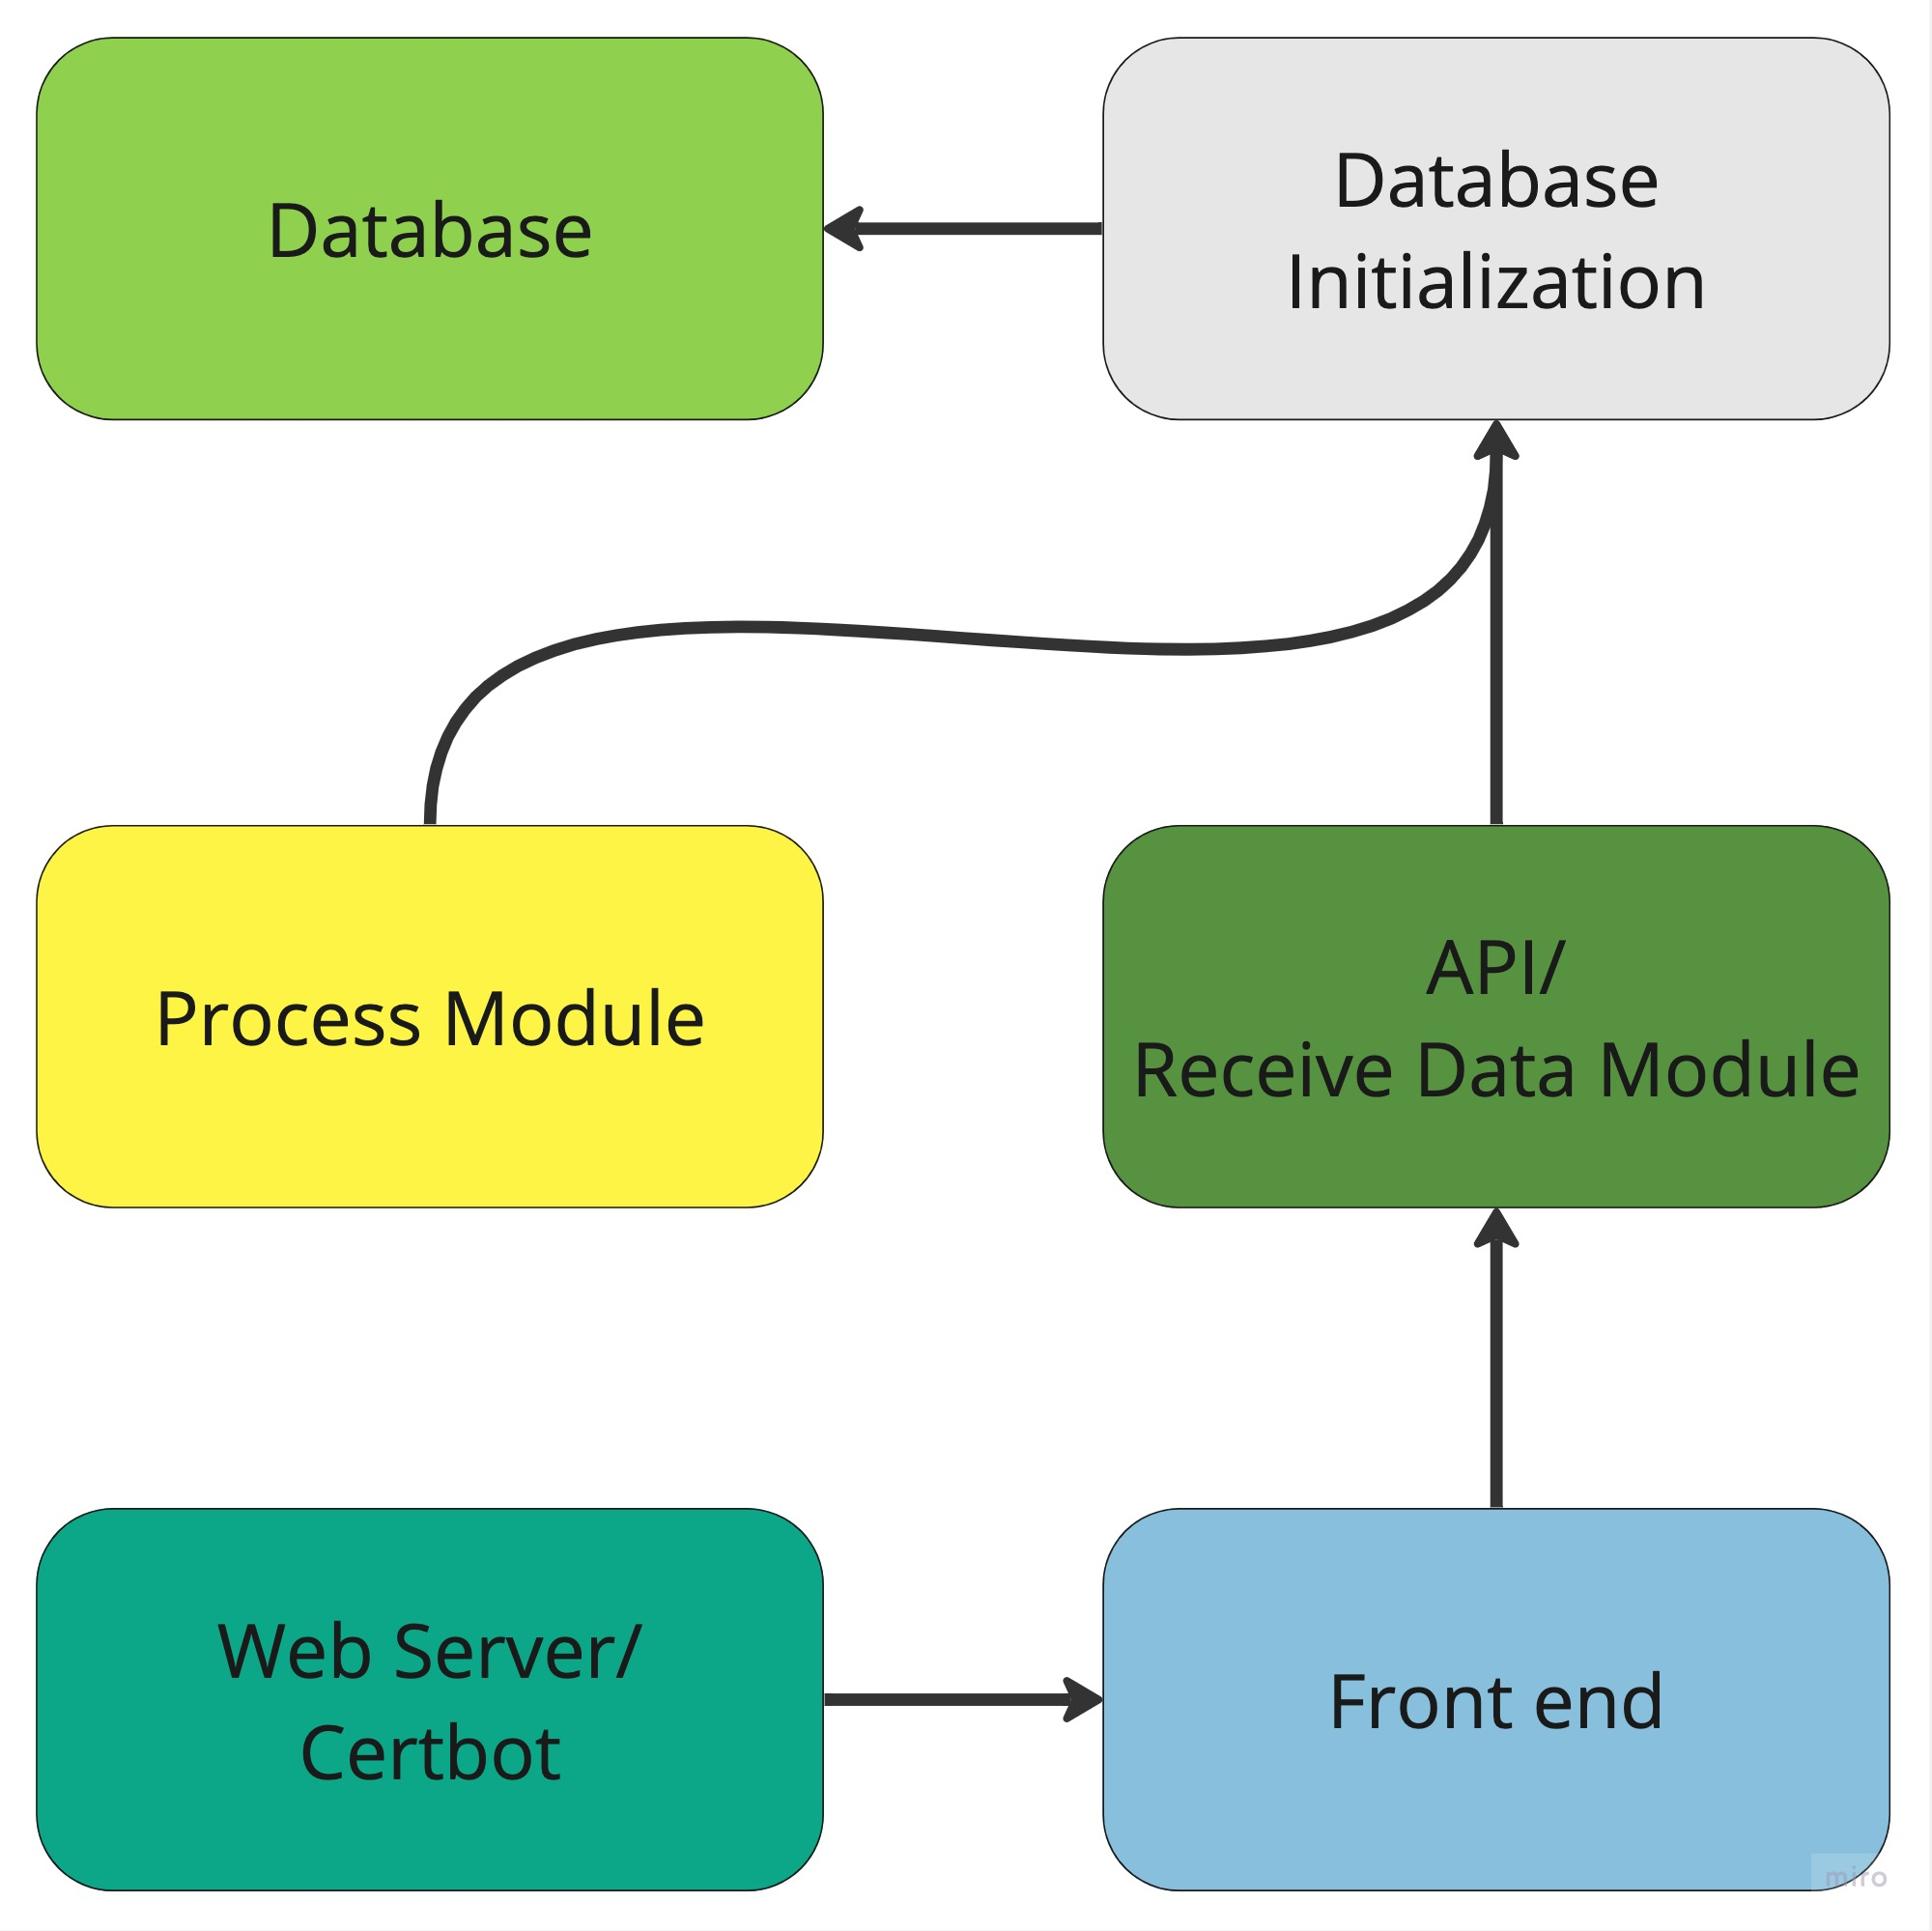
\includegraphics[scale=0.09]{images/containersDependency.jpg}
	\caption{Containers dependency.}
	\label{fig:containersDependencyImpl}
\end{figure}


The Database container uses the MongoDB image to store the project's data. It is configured with root user credentials and mounts the persistent volume \texttt{mongodb\_data\_container} for data storage.

The Database Initialization container is responsible for the initialization and potential population of the database. This container directly depends on the database container to perform its tasks. It uses a custom image, explained in \ref{subsec:containersimagesDefinition}, for this purpose.

The API and data reception module container exposes an API on port 8000. It depends on the database initialization container and connects to the database container using the connection string provided by the internal Docker network.

The data processing module container connects to the database and starts after the Database Initialization container.

The Frontend container directly depends on the API, using the image explained in \label{subsec:containersimages}.

For the container that manages the Web Server using the NGINX image, a periodic restart configuration is made, enabling the SSL certificate to be automatically renewed. It depends on the frontend to start, ensuring that the user interface is available when the server is running.

For the execution of the Web Server, an auxiliary container is used, responsible for the renewal of SSL certificates through \texttt{Certbot} \cite{dockerCertbot}. It is configured to renew the certificates periodically and depends on the frontend, ensuring that the certificate is renewed only when the user interface is available.

The definition of the volume used by the database is explicitly made in the \texttt{docker-compose.yml} file, which is used by the MongoDB container to store data persistently. The network used by the containers is implicitly defined by Docker Compose, which creates a network for the containers and connects them to it, enabling communication between the containers that make up the system.

The \texttt{docker-compose.yml} file that defines the configuration of the containers is in the appendices \ref{containerscompose}.